\chapter{详细设计}
前几章设计了系统的框架、层次、业务对象等方面,本章将对系统进行详尽的设计,包括数据库的设计,主要流程的设计等。
\section{数据库设计}
本系统使用的是MySQL数据库,由于系统框架为微服务框架,所以本章将分模块为设计各自模块的数据库表。同时,为了提高查询速度,便于开发,
所有的数据表均不会设置外键,也没有触发器,全靠后端上层逻辑保证数据的完整性。后期为提高查询速度会设计索引和视图。
\subsection{UserService用户模块}
用户模块的数据表主要设计用户基本信息、角色信息、权限信息等,一方面是为用户登录认证授权服务,另一方面是为管理员进行用户管理服务。权限管理方面采用的是RBAC的数据表设计,即将权限信息分为5个表,
用户信息表、角色信息表、权限信息表、用户角色表和权限角色表。
\subsubsection{User角色表}
\begin{enumerate}
    \item 表结构
    \begin{table}[htbp]
        \centering
        \scalebox{0.8}{
        \begin{tabular}{|l|l|l|l|l|}
        \hline
        字段名          & 字段类型         & 字段描述   & 初始值              & 约束                        \\ \hline
        USER\_ID     & Long         & 用户唯一约束 &                  & PK,AUTO\_INCREMENT        \\ \hline
        CREATE\_TIME & Date         & 创建时间   & CURRENTTIMESTAMP & NULL DEFAULT CURRENTSTAMP \\ \hline
        COUNTRY      & VARCHAR(100) & 国家     &                  &                           \\ \hline
        CITY         & VARCHAR(200) & 城市     &                  &                           \\ \hline
        NAME         & VARHCAR(100) & 姓名     &                  &                             \\ \hline
        IDENTITY\_NO  & VARCHAR(30)  & 身份证   &                  &                             \\ \hline
        \end{tabular}
        }
        \end{table}
    \item 建表语句\\
        CREATE TABLE(\\
            USER\_ID INT(64) PRIMARY KEY AUTO\_INCREMENT,\\
            CREATE\_TIME TIMESTAMP NULL DEFAULT CURRENTTIMESTAMP,\\
            COUNTRY VARCHAR(100),\\
            CITY VARCHAR(200),\\
            NAME VARCHAR(100),\\
            IDENTITY\_NO VARCHAR(30) \\
        )
    \end{enumerate}

\subsubsection{USER\_AUTH用户认证表}
本系统支持第三方登录,所以每个用户对应多个登陆凭证和密码,比如邮箱、手机号等。本表记录的就是用户和对应的登陆方式,包括用户ID、登陆账号、登陆密码、登陆方式等。
\begin{enumerate}
    \item 表结构
    \begin{table}[htbp]
        \centering
        \scalebox{0.8}{
        \begin{tabular}{|l|l|l|l|l|}
        \hline
        \hline
        字段名            & 字段类型         & 字段描述   & 初始值              & 约束                        \\ \hline
        AUTH\_ID       & Long         & 用户唯一约束 &                  & PK,AUTO\_INCREMENT        \\ \hline
        CREATE\_TIME   & Date         & 创建时间   & CURRENTTIMESTAMP & NULL DEFAULT CURRENTSTAMP \\ \hline
        USER\_ID       & Long         & 关联用户标识 &                  & NOT NULL                  \\ \hline
        IDENTITY\_TYPE & int          & 登录类别标识 &                  & NOT NULL                  \\ \hline
        IDENTIFIER     & VARCHAR(50)  & 身份唯一标识 &                  & NOT NULL                  \\ \hline
        CREDENTIAL     & VARCHAR(100) & 登陆验证   &                  & NOT NULL                  \\ \hline
        \end{tabular}
        }
        \end{table}
    \item 建表语句\\
        CREATE TABLE(\\
            AUTH\_ID INT(64) PRIMARY KEY AUTO\_INCREMENT,\\
            USER\_ID INT(64) PRIMARY KEY AUTO\_INCREMENT,\\
            CREATE\_TIME TIMESTAMP NULL DEFAULT CURRENTTIMESTAMP,\\
            IDENTITY\_TYPE INT NOT NULL,\\
            IDENTIFIER VARCHAR(50) NOT NULL,\\
            CREDENTIAL VARCHAR(100) NOT NULL\\
        )
    \end{enumerate}

\subsubsection{DICT\_ROLE角色表}
为了便于权限管理,根据RBAC设计,将多个权限抽象出来,封装在一个角色中。角色表和用户表是多对多的关系,即一个用户可以拥有多个角色,一个角色也可以被多个角色拥有。
\begin{enumerate}
    \item 表结构
    \begin{table}[htbp]
        \centering
        \scalebox{0.8}{
        \begin{tabular}{|l|l|l|l|l|}
        \hline
        \hline
        字段名            & 字段类型         & 字段描述   & 初始值              & 约束                        \\ \hline
        ROLE\_ID     & Long         & 角色唯一约束 &                  & PK,AUTO\_INCREMENT        \\ \hline
        CREATE\_TIME & Date         & 创建时间   & CURRENTTIMESTAMP & NULL DEFAULT CURRENTSTAMP \\ \hline
        ROLE\_NAME   & VARCHAR(30)  & 角色名称   &                  & NOT NULL                  \\ \hline
        DELETE\_MARK & VARCHAR(3)   & 删除标识   & NO               & NULL DEFAULT 'NO'         \\ \hline
        \end{tabular}
        }
        \end{table}
    \item 建表语句\\
        CREATE TABLE(\\
            ROLE\_ID INT(64) PRIMARY KEY AUTO\_INCREMENT,\\
            CREATE\_TIME TIMESTAMP NULL DEFAULT CURRENTTIMESTAMP,\\
            ROLE\_NAME VARCHAR(30) NOT NULL,\\
            DELETE\_MARK VARCHAR(3) NULL DEFAULT 'NO'\\
        )
    \end{enumerate}

\subsubsection{DICT\_PERMISSION权限表}
权限表记载了系统中的所有权限,本系统中的权限值对应的是请求路径,即本系统的权限控制是基于URL的。角色表和权限表是多对多的关系,即一个角色拥有多个权限,一个权限也可以被多个角色拥有。
\begin{enumerate}
    \item 表结构
    \begin{table}[htbp]
        \centering
        \scalebox{0.8}{
        \begin{tabular}{|l|l|l|l|l|}
        \hline
        \hline
        字段名            & 字段类型         & 字段描述   & 初始值              & 约束                        \\ \hline
        PERMISSION\_ID & Long         & 权限唯一约束 &                  & PK,AUTO\_INCREMENT        \\ \hline
        CREATE\_TIME   & Date         & 创建时间   & CURRENTTIMESTAMP & NULL DEFAULT CURRENTSTAMP \\ \hline
        PERMISSION     & VARCHAR(30)  & 权限名称   &                  & NOT NULL                  \\ \hline
        DELETE\_MARK   & VARCHAR(3)   & 删除标识   & NO               & NULL DEFAULT 'NO'         \\ \hline
        \end{tabular}
        }
        \end{table}
    \item 建表语句\\
        CREATE TABLE(\\
            PERMISSION\_ID INT(64) PRIMARY KEY AUTO\_INCREMENT,\\
            CREATE\_TIME TIMESTAMP NULL DEFAULT CURRENTTIMESTAMP,\\
            PERMISSION\_NAME VARCHAR(30) NOT NULL,\\
            DELETE\_MARK VARCHAR(3) NULL DEFAULT 'NO'\\
        )
    \end{enumerate}

\subsubsection{DICT\_USER\_ROLE用户角色表}
此表为用户和角色的关联关系表,将用户id和角色id建立关联,从而可以知道用户对应的角色。
\begin{enumerate}
    \item 表结构
    \begin{table}[htbp]
        \centering
        \scalebox{0.8}{
        \begin{tabular}{|l|l|l|l|l|}
        \hline
        \hline
        字段名            & 字段类型         & 字段描述   & 初始值              & 约束                        \\ \hline
        ROLE\_ID     & INT         & 角色唯一约束 &                  & PK,AUTO\_INCREMENT        \\ \hline
        USER\_ID     & Long         & 用户唯一约束 &                &NOT NULL \\ \hline
        GROUP\_ID    & INT          & 部门ID        & 10005         & NULL DEFAULT 10005  \\ \hline
        CREATE\_TIME & Date         & 创建时间   & CURRENTTIMESTAMP & NULL DEFAULT CURRENTSTAMP \\ \hline
        LOCK\_MARK   & VARCHAR(3)   & 冻结标识   & NO               & NULL DEFAULT 'NO'         \\ \hline
        DELETE\_MARK & VARCHAR(3)   & 删除标识   & NO               & NULL DEFAULT 'NO'         \\ \hline
        \end{tabular}
        }
        \end{table}
    \item 建表语句\\
        CREATE TABLE(\\
            ROLE\_ID INT(64) PRIMARY KEY AUTO\_INCREMENT,\\
            USER\_ID INT(64) NOT NULL, \\
            GROUP\_ID INT NULL DEFAULT 10005, \\
            CREATE\_TIME TIMESTAMP NULL DEFAULT CURRENTTIMESTAMP,\\
            LOCK\_MARK VARCHAR(3) NULL DEFAULT 'NO', \\            
            DELETE\_MARK VARCHAR(3) NULL DEFAULT 'NO'\\
        )
    \end{enumerate}

\subsubsection{DICT\_ROLE\_PERMISSION角色权限表}
此表为角色和权限的关联关系表,将角色id和权限id建立关联,从而可以获取角色对应的权限。
\begin{enumerate}
    \item 表结构
    \begin{table}[htbp]
        \centering
        \scalebox{0.8}{
        \begin{tabular}{|l|l|l|l|l|}
        \hline
        \hline
        字段名            & 字段类型         & 字段描述   & 初始值              & 约束                        \\ \hline
        ID           & INT         & 唯一标识    &                  & PK,AUTO\_INCREMENT        \\ \hline
        ROLE\_ID     & Long         & 角色唯一约束 &                  & NOT NULL        \\ \hline
        PERMISSION\_ID     & Long         & 权限唯一约束 &                &NOT NULL \\ \hline
        CREATE\_TIME & Date         & 创建时间   & CURRENTTIMESTAMP & NULL DEFAULT CURRENTSTAMP \\ \hline
        LOCK\_MARK   & VARCHAR(3)   & 冻结标识   & NO               & NULL DEFAULT 'NO'         \\ \hline
        DELETE\_MARK & VARCHAR(3)   & 删除标识   & NO               & NULL DEFAULT 'NO'         \\ \hline
        \end{tabular}
        }
        \end{table}
    \item 建表语句\\
        CREATE TABLE(\\
            ROLE\_ID INT(64) PRIMARY KEY AUTO\_INCREMENT,\\
            PERMISSION\_ID INT(64) NOT NULL, \\
            CREATE\_TIME TIMESTAMP NULL DEFAULT CURRENTTIMESTAMP,\\
            LOCK\_MARK VARCHAR(3) NULL DEFAULT 'NO', \\            
            DELETE\_MARK VARCHAR(3) NULL DEFAULT 'NO'\\
        )
    \end{enumerate}

\subsubsection{DICT\_MENU栏目表}
本表记录了该系统中当前登录用户可以操作的模块,用于前端动态获取并加载。
\begin{enumerate}
    \item 表结构
    \begin{table}[htbp]
        \centering
        \scalebox{0.8}{
        \begin{tabular}{|l|l|l|l|l|}
        \hline
        \hline
        字段名            & 字段类型         & 字段描述   & 初始值              & 约束                        \\ \hline
        MENU\_ID     & INT                & 唯一约束 &                  & PK,AUTO\_INCREMENT        \\ \hline
        MENU     & VARCHAR(100)       & 栏目名 &                &NOT NULL \\ \hline
        CREATE\_TIME & Date         & 创建时间   & CURRENTTIMESTAMP & NULL DEFAULT CURRENTSTAMP \\ \hline
        URL   & VARCHAR(200)   & 路径   & NO               & NOT NULL         \\ \hline
        DELETE\_MARK & VARCHAR(3)   & 删除标识   & NO               & NULL DEFAULT 'NO'         \\ \hline
        \end{tabular}
        }
        \end{table}
    \item 建表语句\\
        CREATE TABLE(\\
            MENU\_ID INT(64) PRIMARY KEY AUTO\_INCREMENT,\\
            MENU VARCHAR(100) NOT NULL, \\
            CREATE\_TIME TIMESTAMP NULL DEFAULT CURRENTTIMESTAMP,\\
            URL VARCHAR(200) NOT NULL \\            
            DELETE\_MARK VARCHAR(3) NULL DEFAULT 'NO'\\
        )
    \end{enumerate}

\subsubsection{DICT\_ROLE\_MENU角色栏目表}
此表记录了角色和栏目的对应关系,不同角色可以获取不同栏目。
\begin{enumerate}
    \item 表结构
    \begin{table}[htbp]
        \centering
        \scalebox{0.8}{
        \begin{tabular}{|l|l|l|l|l|}
        \hline
        \hline
        字段名            & 字段类型         & 字段描述   & 初始值              & 约束                        \\ \hline
        ID           & INT         & 唯一标识    &                  & PK,AUTO\_INCREMENT        \\ \hline
        ROLE\_ID     & INT         & 角色唯一约束 &                  & NOT NULL        \\ \hline
        MENU\_ID     & INT         & 栏目唯一约束 &                & NOT NULL \\ \hline
        CREATE\_TIME & Date         & 创建时间   & CURRENTTIMESTAMP & NULL DEFAULT CURRENTSTAMP \\ \hline
        DELETE\_MARK & VARCHAR(3)   & 删除标识   & NO               & NULL DEFAULT 'NO'         \\ \hline
        \end{tabular}
        }
        \end{table}
    \item 建表语句\\
        CREATE TABLE(\\
            ROLE\_ID INT(64) PRIMARY KEY AUTO\_INCREMENT,\\
            PERMISSION\_ID INT(64) NOT NULL, \\
            CREATE\_TIME TIMESTAMP NULL DEFAULT CURRENTTIMESTAMP,\\
            LOCK\_MARK VARCHAR(3) NULL DEFAULT 'NO', \\            
            DELETE\_MARK VARCHAR(3) NULL DEFAULT 'NO'\\
        )
    \end{enumerate}

    \subsubsection{DICT\_GROUP部门表}
    此表记录了系统中的所有部门,用于数据权限的管理,不同部门的人之间不能互相看到数据。
    \begin{enumerate}
        \item 表结构
        \begin{table}[htbp]
            \centering
            \scalebox{0.8}{
            \begin{tabular}{|l|l|l|l|l|}
            \hline
            \hline
            字段名            & 字段类型         & 字段描述   & 初始值              & 约束                        \\ \hline
            GROUP\_ID           & INT         & 唯一标识    &                  & PK,AUTO\_INCREMENT        \\ \hline
            GROUP\_NAME     & VARCHAR(200)         & 部门名 &                & NOT NULL \\ \hline
            PARENT\_ID      & INT               & 父级部门         &         & NOT NULL \\ \hline
            CREATE\_TIME & Date         & 创建时间   & CURRENTTIMESTAMP & NULL DEFAULT CURRENTSTAMP \\ \hline
            DELETE\_MARK & VARCHAR(3)   & 删除标识   & NO               & NULL DEFAULT 'NO'         \\ \hline
            \end{tabular}
            }
            \end{table}
        \item 建表语句\\
            CREATE TABLE(\\
                GROUP\_ID INT PRIMARY KEY AUTO\_INCREMENT,\\
                GROUP\_NAME VARCHAR(200) NOT NULL, \\
                CREATE\_TIME TIMESTAMP NULL DEFAULT CURRENTTIMESTAMP,\\
                PARENT\_ID INT NULL NOT NULL, \\            
                DELETE\_MARK VARCHAR(3) NULL DEFAULT 'NO'\\
            )
        \end{enumerate}

\subsubsection{表格关系}
该模块共涉及了9张表,下图~\ref{fig:USER-ER}~为9张表的关系。
\begin{figure}[htbp]
    \centering
    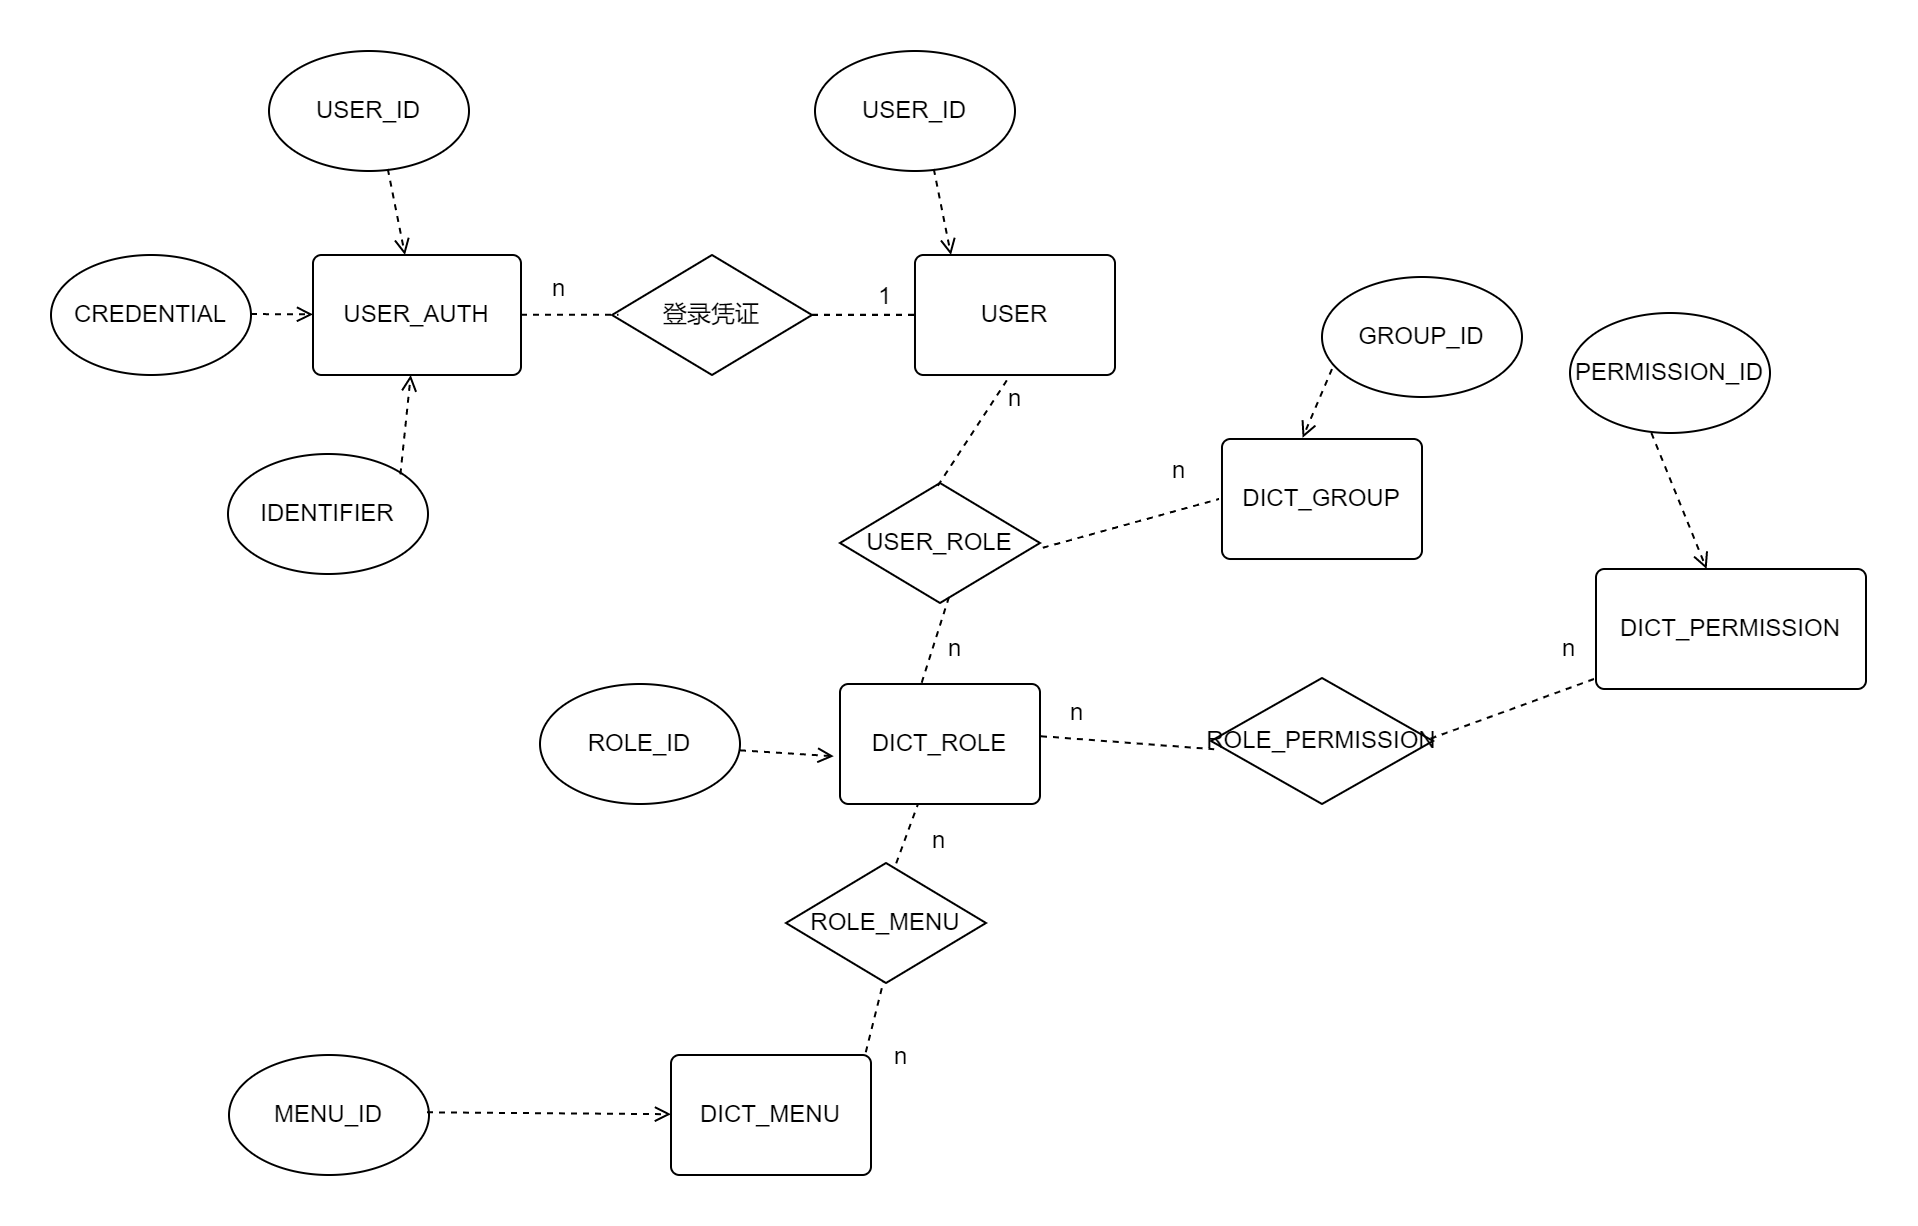
\includegraphics[width=\textwidth]{ch7/USER-ER.jpg}
    \caption{用户管理模块ER图}\label{fig:USER-ER}
    \vspace{\baselineskip} % 表示图与正文空一行
\end{figure}

\subsection{HouseService房源模块}
房源模块主要涉及帖子基本信息、房主联系方式、帖子标签等等和房源帖子相关的数据表。为了功能的扩展性,我们会设置多个字典表,便于功能的增删改,比如标签表的设置是为了方便房源标签的及时增删。
\subsubsection{POST帖子表}
房源帖子包含了帖子的基本信息,比如房源地址、是否允许宠物、房源标签、房源描述等等。
\begin{enumerate}
    \item 表结构
    \begin{table}[htbp]
        \centering
        \scalebox{0.8}{
        \begin{tabular}{|l|l|l|l|l|}
        \hline
        \hline
        字段名            & 字段类型         & 字段描述   & 初始值              & 约束                        \\ \hline
        POST\_ID     & Long         & 帖子唯一约束    &                   & PK,AUTO\_INCREMENT               \\ \hline
        CREATE\_TIME & Date         & 创建时间      & CURRENTTIMESTAMP  & NULL DEFAULT CURRENTSTAMP        \\ \hline
        USER\_ID     & Long         & 关联用户标识    &                   & NOT NULL                         \\ \hline
        DELETE\_MARK & VARCHAR(3)   & 删除标识      & NO                & NULL DEFAULT 'NO'                \\ \hline
        TITLE        & VARCHAR(200) & 标题        & WE CAN OFFER HELP & NULL DEFAULT 'WE CAN OFFER HELP' \\ \hline
        CITY         & VARCHAR(200) & 城市(市,省,国) &                   & NOT NULL                         \\ \hline
        GUESTS       & int          & 人数        & 1                 & NULL DEFAULT 1                   \\ \hline
        PETS         & VARCHAR(3)   & 是否允许宠物    & NO                & NULL DEFAULT 'NO'                \\ \hline
        DURATIONTYPE & int          & 时长类型      & 1                 & NULL DEFAULT 1                   \\ \hline
        TAGS         & VARCHAR(200) & 标签组        &                   &                                  \\ \hline
        ACTIVE       & VARCHAR(3)   & 有效表示      & YES               & NULL DEFAULT 'YES'               \\ \hline
        DESCRIPTION  & VARCHAR(500) & 住所描述
        \end{tabular}
        }
        \end{table}
    \item 建表语句\\
        CREATE TABLE(\\
            POST\_ID INT(64) PRIMARY KEY AUTO\_INCREMENT,\\
            USER\_ID INT(64) NOT NULL, \\
            CREATE\_TIME TIMESTAMP NULL DEFAULT CURRENTTIMESTAMP,\\
            DELETE\_MARK VARCHAR(3) NULL DEFAULT 'NO',\\
            TITLE VARCHAR(200) NULL DEFAULT 'WE CAN OFFER HEPL',\\
            CITY VARCHAR(200) NOT NULL,\\
            GUESTS INT NULL DEFAULT 1,\\
            PETS VARCHAR(3) NULL DEFAULT 'NO',\\
            DURATIONTYPE INT NULL DEFAULT 1,\\
            TAGS VARCHAR(200),\\
            DESCRIPTION VARCHAR(500),\\
            ACTIVE VARCHAR(3) NULL DEFAULT 'YES'\\
        )
    \end{enumerate}

\subsubsection{CONTACT联系方式表}
此表记录了房源帖上具体的联系方式,为了便于联系方式的增删改,我们将联系方式独立出来形成一张数据表,以减少耦合度。表中主要记录了对应的帖子,以及基本的联系信息。
\begin{enumerate}
    \item 表结构
    \begin{table}[htbp]
        \centering
        \scalebox{0.8}{
        \begin{tabular}{|l|l|l|l|l|}
        \hline
        \hline
        字段名            & 字段类型         & 字段描述   & 初始值              & 约束                        \\ \hline
        CONTACT\_ID  & Long         & 唯一约束     &                  & PK,AUTO\_INCREMENT        \\ \hline
        CREATE\_TIME & Date         & 创建时间     & CURRENTTIMESTAMP & NULL DEFAULT CURRENTSTAMP \\ \hline
        POST\_ID     & Long         & 关联关联标识   &                  & NOT NULL                  \\ \hline
        DELETE\_MARK & VARCHAR(3)   & 删除标识     & NO               & NULL DEFAULT 'NO'         \\ \hline
        CONTENT      & VARCHAR(200) & 联系途径     &                  & NOT NULL                  \\ \hline
        TYPE\_ID     & int          & 联系方式类别标识 &                  & NOT NULL                  \\ \hline
        \end{tabular}
        }
        \end{table}
    \item 建表语句\\
        CREATE TABLE(\\
            CONTACT\_ID INT(64) PRIMARY KEY AUTO\_INCREMENT,\\
            POST\_ID INT(64) NOT NULL,\\
            CREATE\_TIME TIMESTAMP NULL DEFAULT CURRENTTIMESTAMP,\\
            DELETE\_MARK VARCHAR(3) NULL DEFAULT 'NO',\\
            CONTENT VARCHAR(200) NOT NULL,\\
            TYPE\_ID INT NOT NULL\\
        )
    \end{enumerate}

\subsubsection{DICT\_CONTACT\_TYPE联系方式类别表}
此表记录了房源帖上那些联系方式的类型,为了后续可以便于直接增加联系方式类型,比如现阶段支持电话和邮箱,一段时间后想增加微信功能,独立出一个类别较容易扩展。
\begin{enumerate}
    \item 表结构
    \begin{table}[htbp]
        \centering
        \scalebox{0.8}{
        \begin{tabular}{|l|l|l|l|l|}
        \hline
        \hline
        字段名            & 字段类型         & 字段描述   & 初始值              & 约束                        \\ \hline
        TYPE\_ID      & int          & 唯一约束     &                  & PK,AUTO\_INCREMENT        \\ \hline
        CREATE\_TIME  & Date         & 创建时间     & CURRENTTIMESTAMP & NULL DEFAULT CURRENTSTAMP \\ \hline
        CONTACT\_NAME & VARCHAR(30)  & 联系方式     &                  & NOT NULL                  \\ \hline
        DELETE\_MARK  & VARCHAR(3)   & 删除标识     & NO               & NULL DEFAULT 'NO'         \\ \hline
        \end{tabular}
        }
        \end{table}
    \item 建表语句\\
        CREATE TABLE(\\
            TYPE\_ID INT PRIMARY KEY AUTO\_INCREMENT,\\
            CREATE\_TIME TIMESTAMP NULL DEFAULT CURRENTTIMESTAMP,\\
            DELETE\_MARK VARCHAR(3) NULL DEFAULT 'NO',\\
            CONTACT\_NAME VARCHAR(30) NOT NULL\\
        )
    \end{enumerate}

\subsubsection{DICT\_TAG标签表}
此表记录了房源帖子上具体的标签,比如标签的类型,标签的内容等。比如说,一个房源帖子的标签为“拥有药物资源,类别为救助”等等。
\begin{enumerate}
    \item 表结构
    \begin{table}[htbp]
        \centering
        \scalebox{0.8}{
        \begin{tabular}{|l|l|l|l|l|}
        \hline
        \hline
        字段名            & 字段类型         & 字段描述   & 初始值              & 约束                        \\ \hline
        TAG\_ID      & int          & 唯一约束     &                  & PK,AUTO\_INCREMENT        \\ \hline
        CREATE\_TIME & Date         & 创建时间     & CURRENTTIMESTAMP & NULL DEFAULT CURRENTSTAMP \\ \hline
        TYPE\_ID     & int          & 标签类别     &                  & NOT NULL                  \\ \hline
        DELETE\_MARK & VARCHAR(3)   & 删除标识     & NO               & NULL DEFAULT 'NO'         \\ \hline
        CONTENT      & VARCHAR(200) & 标签内容     &                  & NOT NULL                  \\ \hline
        \end{tabular}
        }
        \end{table}
    \item 建表语句\\
        CREATE TABLE(\\
            TAG\_ID INT PRIMARY KEY AUTO\_INCREMENT,\\
            CREATE\_TIME TIMESTAMP NULL DEFAULT CURRENTTIMESTAMP,\\
            DELETE\_MARK VARCHAR(3) NULL DEFAULT 'NO',\\
            CONTENT VARCHAR(200) NOT NULL,\\
            TYPE\_ID INT NOT NULL\\
        )
    \end{enumerate}

\subsubsection{DICT\_TAG\_TYPE标签类别表}
每个标签都有对应的类别,这是为了便于管理,也是为了便于扩展,此表记录了标签类别信息,包括类别id、类别内容等。
\begin{enumerate}
    \item 表结构
    \begin{table}[htbp]
        \centering
        \scalebox{0.8}{
        \begin{tabular}{|l|l|l|l|l|}
        \hline
        \hline
        字段名            & 字段类型         & 字段描述   & 初始值              & 约束                        \\ \hline
        TYPE\_ID      & int          & 唯一约束     &                  & PK,AUTO\_INCREMENT        \\ \hline
        CREATE\_TIME  & Date         & 创建时间     & CURRENTTIMESTAMP & NULL DEFAULT CURRENTSTAMP \\ \hline
        TYPE\_NAME    & VARCHAR(50)  & 类别内容     &                  & NOT NULL                  \\ \hline
        DELETE\_MARK  & VARCHAR(3)   & 删除标识     & NO               & NULL DEFAULT 'NO'         \\ \hline
        \end{tabular}
        }
        \end{table}
    \item 建表语句\\
        CREATE TABLE(\\
            TYPE\_ID INT PRIMARY KEY AUTO\_INCREMENT,\\
            CREATE\_TIME TIMESTAMP NULL DEFAULT CURRENTTIMESTAMP,\\
            DELETE\_MARK VARCHAR(3) NULL DEFAULT 'NO',\\
            TYPE\_NAME VARCHAR(50) NOT NULL\\
        )
    \end{enumerate}

\subsubsection{DICT\_DURATION时长类型表}
此表记录了帖子里时长的信息,比如一周、一月、无限期等。
\begin{enumerate}
    \item 表结构
    \begin{table}[htbp]
        \centering
        \scalebox{0.8}{
        \begin{tabular}{|l|l|l|l|l|}
        \hline
        \hline
        字段名            & 字段类型         & 字段描述   & 初始值              & 约束                        \\ \hline
        DURATION\_ID      & int          & 唯一约束     &                  & PK,AUTO\_INCREMENT        \\ \hline
        CREATE\_TIME  & Date         & 创建时间     & CURRENTTIMESTAMP & NULL DEFAULT CURRENTSTAMP \\ \hline
        DURATION    & VARCHAR(50)  & 时长描述     &                  & NOT NULL                  \\ \hline
        DELETE\_MARK  & VARCHAR(3)   & 删除标识     & NO               & NULL DEFAULT 'NO'         \\ \hline
        \end{tabular}
        }
        \end{table}
    \item 建表语句\\
        CREATE TABLE(\\
            DURATION\_ID INT PRIMARY KEY AUTO\_INCREMENT,\\
            CREATE\_TIME TIMESTAMP NULL DEFAULT CURRENTTIMESTAMP,\\
            DELETE\_MARK VARCHAR(3) NULL DEFAULT 'NO',\\
            DURATION VARCHAR(50) NOT NULL\\
        )
    \end{enumerate}


\subsubsection{总体ER图}
本模块的数据表均围绕房源帖子POST展开,下图~\ref{fig:HOUSE-ER}~给出本模块的ER图。
\begin{figure}[htbp]
    \centering
    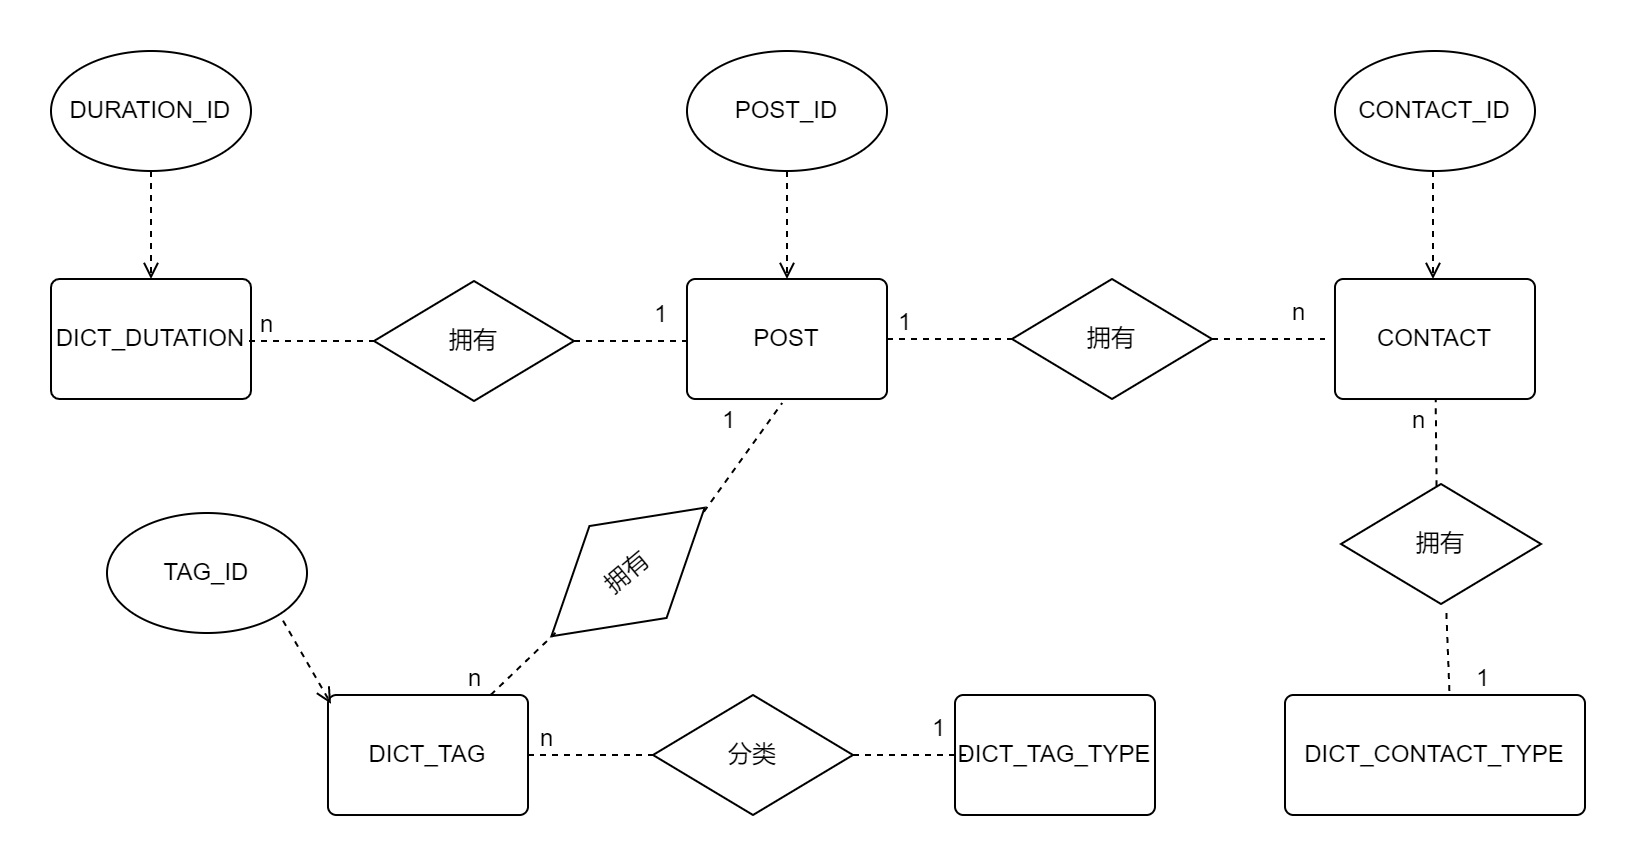
\includegraphics[width=\textwidth]{ch7/HOUSE-ER.jpg}
    \caption{房源管理ER图}\label{fig:HOUSE-ER}
    \vspace{\baselineskip} % 表示图与正文空一行
\end{figure}

\subsection{Report举报模块}
举报模块主要涉及举报基本信息,同时会和其余的模块进行联通,比如用户表、房源帖子表等。
\subsubsection{REPORT举报信息表}
此表记录了举报的基本信息,包括举报内容、举报理由、举报类别、举报人等等。
\begin{enumerate}
    \item 表结构
    \begin{table}[htbp]
        \centering
        \scalebox{0.8}{
        \begin{tabular}{|l|l|l|l|l|}
        \hline
        \hline
        字段名            & 字段类型         & 字段描述   & 初始值              & 约束                        \\ \hline
        REPORT\_ID    & Long         & 唯一约束 &                  & PK,AUTO\_INCREMENT        \\ \hline
        CREATE\_TIME  & Date         & 创建时间 & CURRENTTIMESTAMP & NULL DEFAULT CURRENTSTAMP \\ \hline
        OBJTYPE\_ID    & int          & 举报类型 &                  & NOT NULL                  \\ \hline
        DELETE\_MARK  & VARCHAR(3)   & 删除标识 & NO               & NULL DEFAULT 'NO'         \\ \hline
        DEFENSE       & Long         & 被举报者 &                  & NOT NULL                  \\ \hline
        RESON         & VARCHAR(500) & 举报利用 &                  & NOT NULL                  \\ \hline
        PROSECUTION   & Long         & 举报者  &                  & NOT NULL                  \\ \hline
        AUDIT\_STATUS & int          & 审核状态 & 1                & NULL DEFAULT 1            \\ \hline
        \end{tabular}
        }
        \end{table}
    \item 建表语句\\
        CREATE TABLE(\\
            REPORT\_ID INT(64) PRIMARY KEY AUTO\_INCREMENT,\\
            CREATE\_TIME TIMESTAMP NULL DEFAULT CURRENTTIMESTAMP,\\
            DELETE\_MARK VARCHAR(3) NULL DEFAULT 'NO',\\
            OBJTYPE\_ID INT NOT NULL,\\
            DEFENSE INT(64) NOT NULL,\\
            RESON VARCHAR(500) NOT NULL,\\
            PROSECUTION LONG NOT NULL,\\
            AUDIT\_STATUS INT NULL DEFAULT 1\\
        )
    \end{enumerate}

\subsection{AUDIT模块}
该模块为本系统的审核模块,记录的信息有审核的基本信息、审核类别等,目的是将系统的历次审核记录下来形成日志,便于管理。】
\subsubsection{AUDIT审核表}
此表记录了审核的基本信息,包括审核内容、操作人、操作类型等等。
\begin{enumerate}
    \item 表结构
    \begin{table}[htbp]
        \centering
        \scalebox{0.8}{
        \begin{tabular}{|l|l|l|l|l|}
        \hline
        \hline
        字段名            & 字段类型         & 字段描述   & 初始值              & 约束                        \\ \hline
        AUDIT\_ID      & Long          & 唯一约束     &                  & PK,AUTO\_INCREMENT        \\ \hline
        CREATE\_TIME  & Date         & 创建时间     & CURRENTTIMESTAMP & NULL DEFAULT CURRENTSTAMP \\ \hline
        OBJTYPE\_ID      & int  & 被审核类别     &                  & NOT NULL                  \\ \hline
        DELETE\_MARK  & VARCHAR(3)   & 删除标识     & NO               & NULL DEFAULT 'NO'         \\ \hline
        STATUS        & int  & 审核状态     & 1    & NULL DEFAULT 1 \\ \hline
        OPERATOR      & Long  & 审核人       &      & NOT NULL \\ \hline
        OPER          & int   & 操作        &       & NOT NULL \\ \hline
        MESSAGE       & VARCHAR(200)    &       & \\ \hline
        \end{tabular}
        }
        \end{table}
    \item 建表语句\\
        CREATE TABLE(\\
            AUDIT\_ID INT PRIMARY KEY AUTO\_INCREMENT,\\
            CREATE\_TIME TIMESTAMP NULL DEFAULT CURRENTTIMESTAMP,\\
            DELETE\_MARK VARCHAR(3) NULL DEFAULT 'NO',\\
            OBJTYPE\_ID INT NOT NULL,\\
            STATUS  INT NOT NULL,\\
            OPERATOR LONG NOT NULL,\\
            OPER INT NOT NULL,\\
            MESSAGE VARCHAR(200) \\
        )
    \end{enumerate}

\subsubsection{DICT\_OPER\_TYPE审核类型表}
此表表示所有业务对象的审核类型,包括管理员通过、管理员驳回等,便于管理和扩展。
\begin{enumerate}
    \item 表结构
    \begin{table}[htbp]
        \centering
        \scalebox{0.8}{
        \begin{tabular}{|l|l|l|l|l|}
        \hline
        \hline
        字段名            & 字段类型         & 字段描述   & 初始值              & 约束                        \\ \hline
        OPER\_ID      & int          & 唯一约束     &                  & PK,AUTO\_INCREMENT        \\ \hline
        CREATE\_TIME  & Date         & 创建时间     & CURRENTTIMESTAMP & NULL DEFAULT CURRENTSTAMP \\ \hline
        DELETE\_MARK  & VARCHAR(3)   & 删除标识     & NO               & NULL DEFAULT 'NO'         \\ \hline
        OPER          & VARCHAR(200)   & 操作        &       & NOT NULL \\ \hline
        \end{tabular}
        }
        \end{table}
    \item 建表语句\\
        CREATE TABLE(\\
            OPER\_ID INT PRIMARY KEY AUTO\_INCREMENT,\\
            CREATE\_TIME TIMESTAMP NULL DEFAULT CURRENTTIMESTAMP,\\
            DELETE\_MARK VARCHAR(3) NULL DEFAULT 'NO',\\
            OPER VARCHAR(200) NOT NULL \\
        )
    \end{enumerate}


    \subsubsection{DICT\_STATUS审核状态表}
    此表标识所有业务对象的审核状态,包括待审核、驳回、通过等。
    \begin{enumerate}
        \item 表结构
        \begin{table}[htbp]
            \centering
            \scalebox{0.8}{
            \begin{tabular}{|l|l|l|l|l|}
            \hline
            \hline
            字段名            & 字段类型         & 字段描述   & 初始值              & 约束                        \\ \hline
            STATUS\_ID    & int         & 唯一约束 &                  & PK,AUTO\_INCREMENT        \\ \hline
            CREATE\_TIME  & Date         & 创建时间 & CURRENTTIMESTAMP & NULL DEFAULT CURRENTSTAMP \\ \hline
            STATUS    & VARCHAR(30)         & 状态 &                  & NOT NULL                  \\ \hline
            DELETE\_MARK  & VARCHAR(3)   & 删除标识 & NO               & NULL DEFAULT 'NO'         \\ \hline
            \end{tabular}
            }
            \end{table}
        \item 建表语句\\
            CREATE TABLE(\\
                STATUS\_ID INT(64) PRIMARY KEY AUTO\_INCREMENT,\\
                CREATE\_TIME TIMESTAMP NULL DEFAULT CURRENTTIMESTAMP,\\
                DELETE\_MARK VARCHAR(3) NULL DEFAULT 'NO',\\
                STATUS VARCHAR(30) NOT NULL\\
            )
        \end{enumerate}

\subsubsection{总体ER图}
本模块的总体ER图如图~\ref{fig:AUDIT-ER}所示
\begin{figure}[htbp]
    \centering
    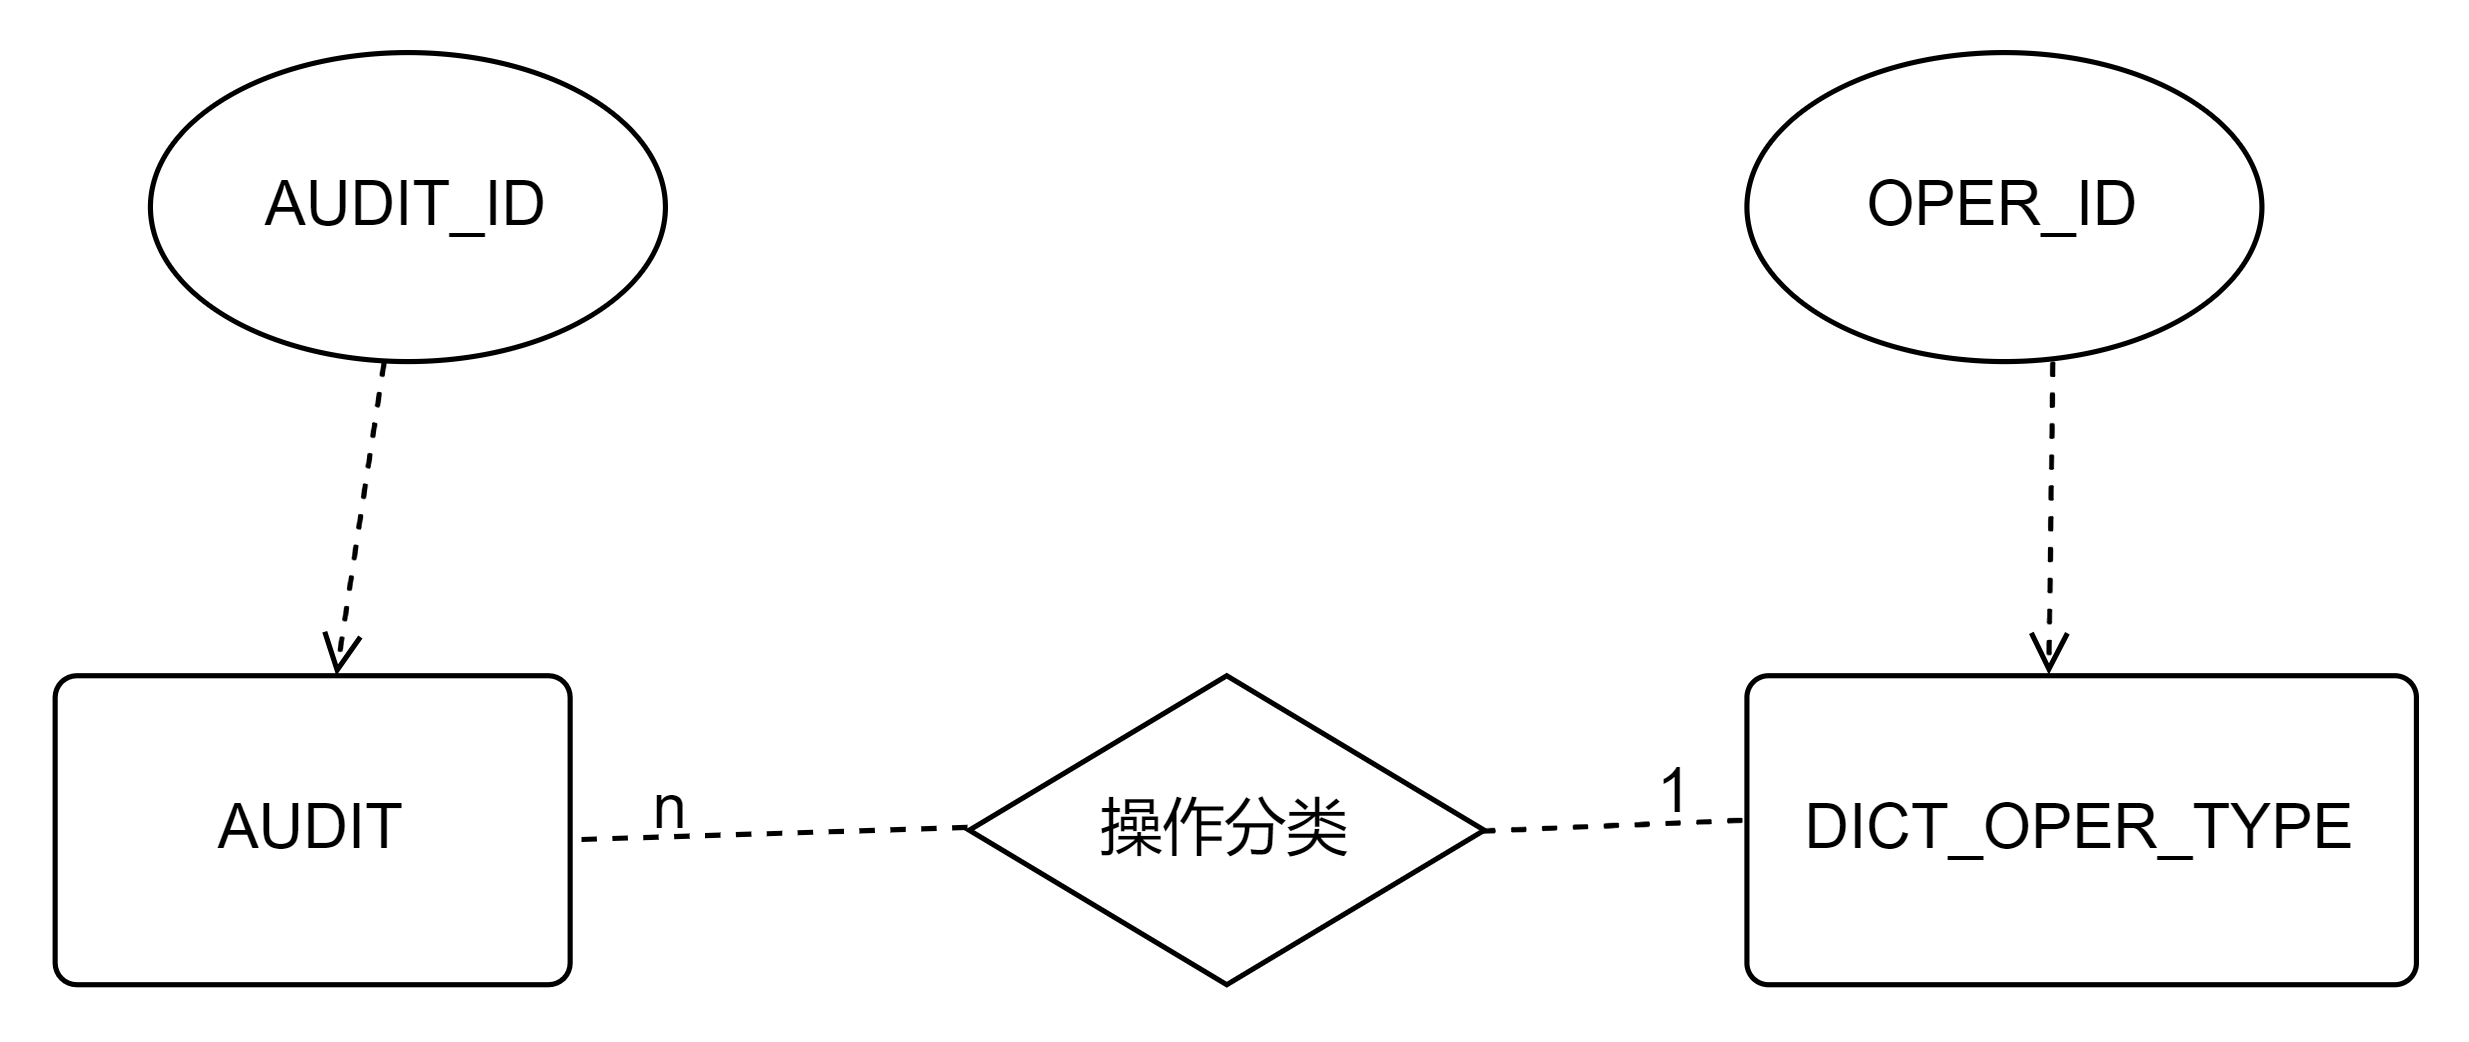
\includegraphics[width=\textwidth]{ch7/AUDIT-ER.jpg}
    \caption{审核模块ER图}\label{fig:AUDIT-ER}
    \vspace{\baselineskip} % 表示图与正文空一行
\end{figure}

\subsection{News模块}
News是新闻模块,涉及到的数据表有新闻基本信息表,新闻内容表,新闻栏目表等。
\subsubsection{NEWS新闻基本信息表}
本表记录了新闻的基本信息,包括新闻的标题、栏目、阅读量等等。
\begin{enumerate}
    \item 表结构
    \begin{table}[htbp]
        \centering
        \scalebox{0.8}{
        \begin{tabular}{|l|l|l|l|l|}
        \hline
        \hline
        字段名            & 字段类型         & 字段描述   & 初始值              & 约束                        \\ \hline
        NEWS\_ID      & Long          & 唯一约束     &                  & PK,AUTO\_INCREMENT        \\ \hline
        CREATE\_TIME  & Date         & 创建时间     & CURRENTTIMESTAMP & NULL DEFAULT CURRENTSTAMP \\ \hline
        DELETE\_MARK  & VARCHAR(3)   & 删除标识     & NO               & NULL DEFAULT 'NO'         \\ \hline
        CATALOGUE     & int          & 栏目        &       & NOT NULL \\ \hline
        TITLE         & VARCHAR(200) & 标题        &       & NOT NULL \\ \hline
        AUTHORS       & VARCHAR(200) & 作者        &       & NOT NULL \\ \hline
        LINK          & VARCHAR(500) & 引用链接    &        &       \\ \hline
        UPDATE\_TIME  & Date         & 修改日期    & CURRENTTIMESTAMP & NULL DEFAULT CURRENTTIMESTAMP \\ \hline
        READ\_NUM     & int          & 阅读量      & 0      & NULL DEFAULT 0 \\ \hline
        STATUS        & int          & 状态        & 1      & NULL DEFAULT 1  \\ \hline
        \end{tabular}
        }
        \end{table}
    \item 建表语句\\
        CREATE TABLE(\\
            NEWS\_ID INT PRIMARY KEY AUTO\_INCREMENT,\\
            CREATE\_TIME TIMESTAMP NULL DEFAULT CURRENTTIMESTAMP,\\
            DELETE\_MARK VARCHAR(3) NULL DEFAULT 'NO',\\
            CATALOGUE INT NOT NULL ,\\
            TITLE VATCHAR(200) NOT NULL,\\
            AUTHORS VARCHAR(200) NOT NULL,\\
            LINK VARCHAR(200) ,\\
            UPDATE\_TIME TIMESTAMP NULL DEFAULT CURRENTTIMESTAMP,\\
            READ\_NUM INT NULL DEFAULT 0,\\
            STATUS INT NULL DEFAULT 1\\
        )
    \end{enumerate}

\subsubsection{NEWS\_PIC新闻图片表}
本表记录了新闻信息中的图片信息,表中保存了图片的链接地址、大小、文件名等信息。
\begin{enumerate}
    \item 表结构
    \begin{table}[htbp]
        \centering
        \scalebox{0.8}{
        \begin{tabular}{|l|l|l|l|l|}
        \hline
        \hline
        字段名            & 字段类型         & 字段描述   & 初始值              & 约束                        \\ \hline
        PIC\_ID      & Long          & 唯一约束     &                  & PK,AUTO\_INCREMENT        \\ \hline
        NEWS\_ID      & Long         & 新闻标识     &                  & NOT NULL \\ \hline
        CREATE\_TIME  & Date         & 创建时间     & CURRENTTIMESTAMP & NULL DEFAULT CURRENTSTAMP \\ \hline
        DELETE\_MARK  & VARCHAR(3)   & 删除标识     & NO               & NULL DEFAULT 'NO'         \\ \hline
        PIC\_NAME     & VARCHAR(100)          & 图片名称        &       & NOT NULL \\ \hline
        FILE\_NAME    & VARCHAR(200) & 文件名        &       & NOT NULL \\ \hline
        FILE\_SIZE    & int          & 大小        &       & NOT NULL \\ \hline
        PIC\_DES          & VARCHAR(500) & 描述    &        &        \\ \hline
        FILE\_PATH     & VARCHAR(200)    & 目录      &       & NOT NULL \\ \hline
        \end{tabular}
        }
        \end{table}
    \item 建表语句\\
        CREATE TABLE(\\
            PIC\_ID INT(64) PRIMARY KEY AUTO\_INCREMENT,\\
            NEW\_ID INT(64) NOT NULL,\\
            CREATE\_TIME TIMESTAMP NULL DEFAULT CURRENTTIMESTAMP,\\
            DELETE\_MARK VARCHAR(3) NULL DEFAULT 'NO',\\
            PIC\_NAME VARCHAR(100) NOT NULL ,\\
            FILE\_NAME VATCHAR(200) NOT NULL,\\
            FILE\_SIZE INT NOT NULL,\\
            PIC\_DES VARCHAR(500) ,\\
            FILE\_PATH VARCHAR(200) NOT NULL\\
        )
    \end{enumerate}

\subsubsection{NEWS\_CONTENT新闻文本表}
此表记录了新闻的文本信息,本系统的文本系统拟定使用MarkDown格式,表中记录了对应的新闻,文本文件的位置等。
\begin{enumerate}
    \item 表结构
    \begin{table}[htbp]
        \centering
        \scalebox{0.8}{
        \begin{tabular}{|l|l|l|l|l|}
        \hline
        \hline
        字段名            & 字段类型         & 字段描述   & 初始值              & 约束                        \\ \hline
        CONTENT\_ID      & Long          & 唯一约束     &                  & PK,AUTO\_INCREMENT        \\ \hline
        NEWS\_ID      & Long         & 新闻标识     &                  & NOT NULL \\ \hline
        CREATE\_TIME  & Date         & 创建时间     & CURRENTTIMESTAMP & NULL DEFAULT CURRENTSTAMP \\ \hline
        DELETE\_MARK  & VARCHAR(3)   & 删除标识     & NO               & NULL DEFAULT 'NO'         \\ \hline
        FILE\_NAME    & VARCHAR(200) & 文件名        &       & NOT NULL \\ \hline
        FILE\_SIZE    & int          & 大小        &       & NOT NULL \\ \hline
        FILE\_PATH     & VARCHAR(200)    & 目录      &       & NOT NULL \\ \hline
        \end{tabular}
        }
        \end{table}
    \item 建表语句\\
        CREATE TABLE(\\
            CONTENT\_ID INT(64) PRIMARY KEY AUTO\_INCREMENT,\\
            NEW\_ID INT(64) NOT NULL,\\
            CREATE\_TIME TIMESTAMP NULL DEFAULT CURRENTTIMESTAMP,\\
            DELETE\_MARK VARCHAR(3) NULL DEFAULT 'NO',\\
            FILE\_NAME VATCHAR(200) NOT NULL,\\
            FILE\_SIZE INT NOT NULL,\\
            FILE\_PATH VARCHAR(200) NOT NULL\\
        )
    \end{enumerate}

\subsubsection{DICT\_CATALOGUE新闻栏目类}
此表记录了新闻的栏目集合,包括栏目名称、创建日期等。
\begin{enumerate}
    \item 表结构
    \begin{table}[htbp]
        \centering
        \scalebox{0.8}{
        \begin{tabular}{|l|l|l|l|l|}
        \hline
        \hline
        字段名            & 字段类型         & 字段描述   & 初始值              & 约束                        \\ \hline
        CATALOGUE\_ID      & int          & 唯一约束     &                  & PK,AUTO\_INCREMENT        \\ \hline
        CREATE\_TIME  & Date         & 创建时间     & CURRENTTIMESTAMP & NULL DEFAULT CURRENTSTAMP \\ \hline
        DELETE\_MARK  & VARCHAR(3)   & 删除标识     & NO               & NULL DEFAULT 'NO'         \\ \hline
        CATALOGUE          & VARCHAR(30)   & 栏目        &       & NOT NULL \\ \hline
        \end{tabular}
        }
        \end{table}
    \item 建表语句\\
        CREATE TABLE(\\
            CATALOGUE\_ID INT PRIMARY KEY AUTO\_INCREMENT,\\
            CREATE\_TIME TIMESTAMP NULL DEFAULT CURRENTTIMESTAMP,\\
            DELETE\_MARK VARCHAR(3) NULL DEFAULT 'NO',\\
            CATALOGUE VARCHAR(30) NOT NULL \\
        )
    \end{enumerate}

\subsubsection{总体ER图}
如图~\ref{fig:NEWS-ER}~所示为NEWS模块的总体ER图。
\begin{figure}[htbp]
    \centering
    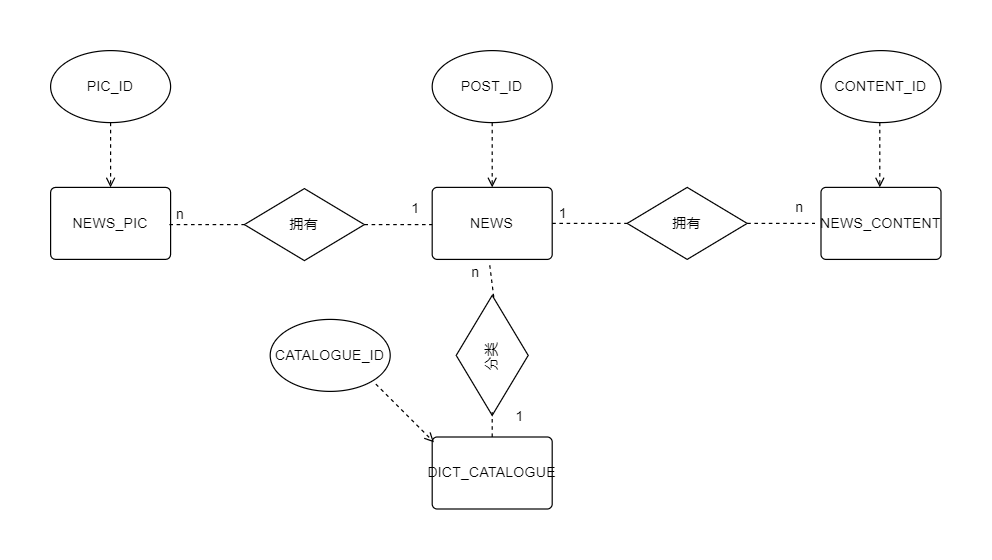
\includegraphics[width=\textwidth]{ch7/NEWS-ER.jpg}
    \caption{新闻模块ER图}\label{fig:NEWS-ER}
    \vspace{\baselineskip} % 表示图与正文空一行
\end{figure}

\subsection{SystemService模块}
该模块为系统管理模块,保存系统相关的数据,比如业务对象类型、系统信息、系统日志等。
\subsubsection{DICT\_OBJTYPE业务对象表}
本表记录了本系统中用到的所有业务对象,并将其进行分类,便于管理和业务对象的扩展。
\begin{enumerate}
    \item 表结构
    \begin{table}[htbp]
        \centering
        \scalebox{0.8}{
        \begin{tabular}{|l|l|l|l|l|}
        \hline
        \hline
        字段名            & 字段类型         & 字段描述   & 初始值              & 约束                        \\ \hline
        OBJTYPE\_ID      & int          & 唯一约束     &                  & PK,AUTO\_INCREMENT        \\ \hline
        CREATE\_TIME  & Date         & 创建时间     & CURRENTTIMESTAMP & NULL DEFAULT CURRENTSTAMP \\ \hline
        DELETE\_MARK  & VARCHAR(3)   & 删除标识     & NO               & NULL DEFAULT 'NO'         \\ \hline
        OBJTYPE          & VARCHAR(100)   & 操作        &       & NOT NULL \\ \hline
        \end{tabular}
        }
        \end{table}
    \item 建表语句\\
        CREATE TABLE(\\
            OBJTYPE\_ID INT PRIMARY KEY AUTO\_INCREMENT,\\
            CREATE\_TIME TIMESTAMP NULL DEFAULT CURRENTTIMESTAMP,\\
            DELETE\_MARK VARCHAR(3) NULL DEFAULT 'NO',\\
            OBJTYPE VARCHAR(200) NOT NULL \\
        )
    \end{enumerate}

\subsubsection{MESSAGE系统信息表}
本表记录了系统消息类,具体包括消息类别、消息人群、操作人等。
\begin{enumerate}
    \item 表结构
    \begin{table}[htbp]
        \centering
        \scalebox{0.8}{
        \begin{tabular}{|l|l|l|l|l|}
        \hline
        \hline
        字段名            & 字段类型         & 字段描述   & 初始值              & 约束                        \\ \hline
        MESSAGE\_ID      & Long          & 唯一约束     &                  & PK,AUTO\_INCREMENT        \\ \hline
        CREATE\_TIME  & Date         & 创建时间     & CURRENTTIMESTAMP & NULL DEFAULT CURRENTSTAMP \\ \hline
        DELETE\_MARK  & VARCHAR(3)   & 删除标识     & NO               & NULL DEFAULT 'NO'         \\ \hline
        CONTENT          & VARCHAR(1000)   & 内容        &       & NOT NULL \\ \hline
        SCOPE          & int            & 范围          &           & NOT NULL \\ \hline
        SPECIFIC\_USERS & VARCHAR(4000) & 特定人群     &            & \\ \hline
        TITLE           & VARCHAR(100)  & 标题          &           & NOT NULL \\ \hline
        \end{tabular}
        }
        \end{table}
    \item 建表语句\\
        CREATE TABLE(\\
            MESSAGE\_ID INT(64) PRIMARY KEY AUTO\_INCREMENT,\\
            CREATE\_TIME TIMESTAMP NULL DEFAULT CURRENTTIMESTAMP,\\
            DELETE\_MARK VARCHAR(3) NULL DEFAULT 'NO',\\
            CONTENT VARCHAR(1000) NOT NULL, \\
            SCOPE INT NOT NULL,\\
            SPECIFIC\_USERS VARCHAR(4000),\\
            TITLE VARCHAR(100) NOT NULL\\
        )
    \end{enumerate}

\subsubsection{DICT\_SCOPE消息范围表}
本表记录了系统模块消息记录的发送范围,以便管理。
\begin{enumerate}
    \item 表结构
    \begin{table}[htbp]
        \centering
        \scalebox{0.8}{
        \begin{tabular}{|l|l|l|l|l|}
        \hline
        \hline
        字段名            & 字段类型         & 字段描述   & 初始值              & 约束                        \\ \hline
        SCOPE\_ID      & Long          & 唯一约束     &                  & PK,AUTO\_INCREMENT        \\ \hline
        CREATE\_TIME  & Date         & 创建时间     & CURRENTTIMESTAMP & NULL DEFAULT CURRENTSTAMP \\ \hline
        DELETE\_MARK  & VARCHAR(3)   & 删除标识     & NO               & NULL DEFAULT 'NO'         \\ \hline
        SCOPE          & VARCHAR(100)   & 范围        &       & NOT NULL \\ \hline
            \end{tabular}
        }
        \end{table}
    \item 建表语句\\
        CREATE TABLE(\\
            SCOPE\_ID INT(64) PRIMARY KEY AUTO\_INCREMENT,\\
            CREATE\_TIME TIMESTAMP NULL DEFAULT CURRENTTIMESTAMP,\\
            DELETE\_MARK VARCHAR(3) NULL DEFAULT 'NO',\\
            SCOPE VARCHAR(100) NOT NULL\\
        )
    \end{enumerate}

\subsubsection{SYSLOG系统日志表}
本表记录了系统模块管理员所进行的一些重要操作,比如修改用户信息、修改新闻信息等等。本表信息包含了日志的操作类型、操作时间、板块类型等等。
\begin{enumerate}
    \item 表结构
    \begin{table}[htbp]
        \centering
        \scalebox{0.8}{
        \begin{tabular}{|l|l|l|l|l|}
        \hline
        \hline
        字段名            & 字段类型         & 字段描述   & 初始值              & 约束                        \\ \hline
        LOG\_ID      & Long          & 唯一约束     &                  & PK,AUTO\_INCREMENT        \\ \hline
        CREATE\_TIME  & Date         & 创建时间     & CURRENTTIMESTAMP & NULL DEFAULT CURRENTSTAMP \\ \hline
        DELETE\_MARK  & VARCHAR(3)   & 删除标识     & NO               & NULL DEFAULT 'NO'         \\ \hline
        OBJTYPE\_ID          & int   & 业务对象类型        &       & NOT NULL \\ \hline
        OBJ\_ID        & Long       & 业务对象标识      &              & NOT NULL \\ \hline
        OPERATOR      & Long        & 操作人            &           & NOT NULL \\ \hline
        OPERATION      & int        & 操作              &           & NOT NULL \\ \hline
        MESSAGE         & VARCHAR(200)  & 操作说明         &        & NOT NULL \\ \hline
            \end{tabular}
        }
        \end{table}
    \item 建表语句\\
        CREATE TABLE(\\
            LOG\_ID INT(64) PRIMARY KEY AUTO\_INCREMENT,\\
            CREATE\_TIME TIMESTAMP NULL DEFAULT CURRENTTIMESTAMP,\\
            DELETE\_MARK VARCHAR(3) NULL DEFAULT 'NO',\\
            OBJTYPE\_ID INT NOT NULL,\\
            OBJ\_ID INT(64) NOT NULL,\\
            OPERATOR INT(64) NOT NULL, \\
            OPERATION INT NOT NULL, \\
            MESSAGE VARCHAR(200) NOT NULL\\
        )
    \end{enumerate}

\subsubsection{DICT\_SYS\_OPERATION}
本表记录了系统管理模块对应着的一切操作类型,主要包含重要模块信息的增删改查。
\begin{enumerate}
    \item 表结构
    \begin{table}[htbp]
        \centering
        \scalebox{0.8}{
        \begin{tabular}{|l|l|l|l|l|}
        \hline
        \hline
        字段名            & 字段类型         & 字段描述   & 初始值              & 约束                        \\ \hline
        OPER\_ID      & int          & 唯一约束     &                  & PK,AUTO\_INCREMENT        \\ \hline
        CREATE\_TIME  & Date         & 创建时间     & CURRENTTIMESTAMP & NULL DEFAULT CURRENTSTAMP \\ \hline
        DELETE\_MARK  & VARCHAR(3)   & 删除标识     & NO               & NULL DEFAULT 'NO'         \\ \hline
        OPER          & VARCHAR(200)   & 操作        &       & NOT NULL \\ \hline
        \end{tabular}
        }
        \end{table}
    \item 建表语句\\
        CREATE TABLE(\\
            OPER\_ID INT PRIMARY KEY AUTO\_INCREMENT,\\
            CREATE\_TIME TIMESTAMP NULL DEFAULT CURRENTTIMESTAMP,\\
            DELETE\_MARK VARCHAR(3) NULL DEFAULT 'NO',\\
            OPER VARCHAR(200) NOT NULL \\
        )
    \end{enumerate}

\section{重要流程设计}
对于系统中的重要操作的后端逻辑流程,接下来进行详细的设计。重要逻辑流程,多为各个服务模块之间的先后调用,本节将使用时序图
展示服务调用先后关系,比如用户登录、用户授权、用户发帖等等流程。

\subsection{登录授权流程}
登录是用户使用产品的开始,也是认证授权的开始,由于本系统采用的是微服务模块,各个模块之间独立部署,若是每个模块都集成登录功能,则太过冗余,
若是在网关负责登录授权,一则网关负担过重,二则一旦网关攻破,内部会很危险,所以特意独立出一个认证授权服务专门负责此功能,同时采用JWT进行用户身份认证。

具体流程为:
\begin{itemize}
    \item 用户请求登录接口,网关转发请求至用户认证模块,若认证成功则返回登录凭证token,并将用户权限存于Redis缓存,否则返回失败信息。
    \item 用户请求其余功能,网关检查是否携带token,若无token则返回登陆提示,若有将token发送至授权模块。
    \item 授权模块获取token,解析用户信息,获取用户权限,检验权限,并返回检验结果给网关。
    \item 若用户有权限,则网关转发请求至对应服务,若没有权限,则返回权限不足信息。
\end{itemize}

下图图~\ref{fig:login}~为时序图:
\begin{figure}[htbp]
    \centering
    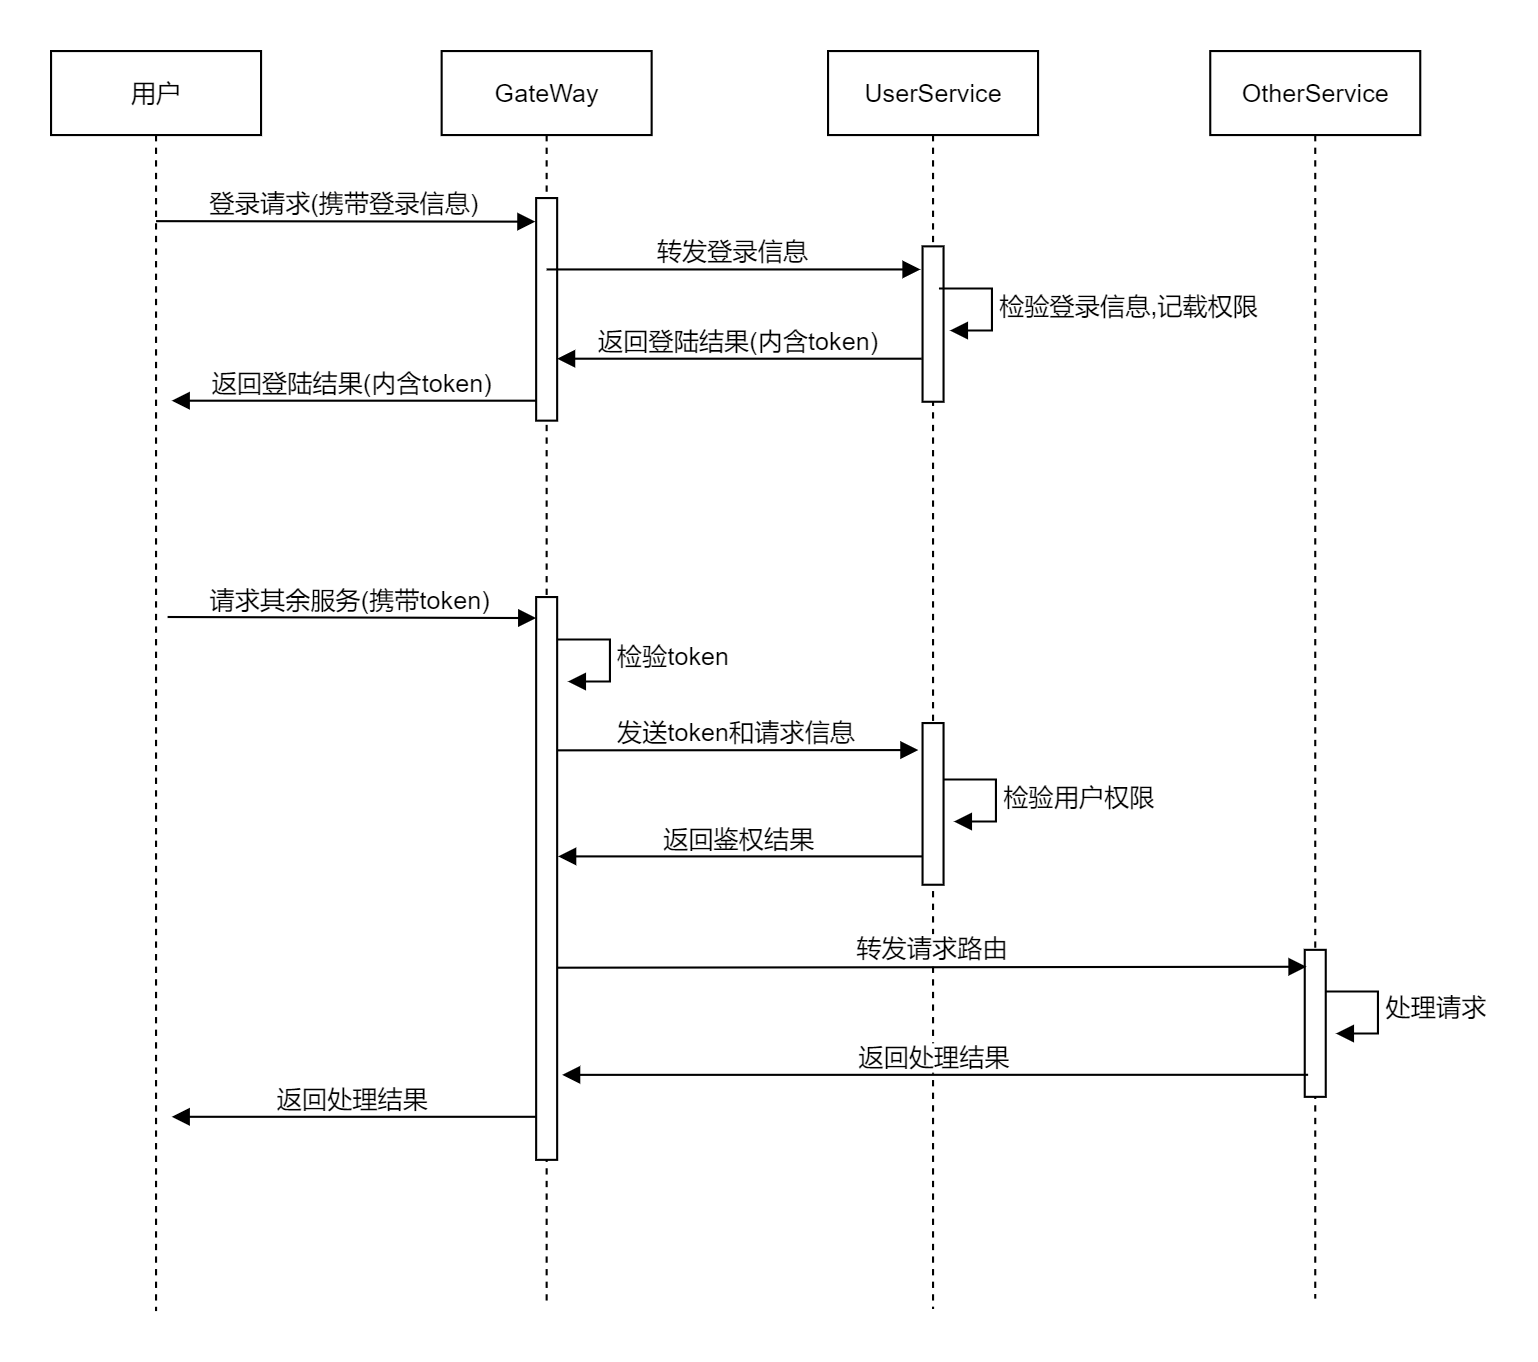
\includegraphics[width=\textwidth]{ch7/login.jpg}
    \caption{登录授权}\label{fig:login}
    \vspace{\baselineskip} % 表示图与正文空一行
\end{figure}

\subsection{用户邮箱注册}
用户系统支持用户邮箱注册,邮箱注册需要用户输入自己的邮箱号,和预设的密码,以及基本的用户信息。提交注册申请后,后台会给用户发送检验邮件,
用户需要打开自己的邮箱进行激活操作。

具体流程为:
\begin{itemize}
    \item 用户请求注册接口,网关转发注册信息至用户管理模块。
    \item 用户管理模块检验参数合法性,若参数不合法则返回注册失败,若合法则生成密钥,存入Redis缓存,并将密钥嵌入邮件发送给注册邮箱。
    \item 用户打开邮箱点击激活链接进行激活,实际是一条携带密钥的激活请求,网关转发至用户管理模块。
    \item 用户管理检验密钥是否和缓存的匹配,若匹配则写入数据库,并返回注册成功,若不匹配或者是超过时限则返回注册失败。
\end{itemize}

下图图~\ref{fig:register}~为时序图:
\begin{figure}[htbp]
    \centering
    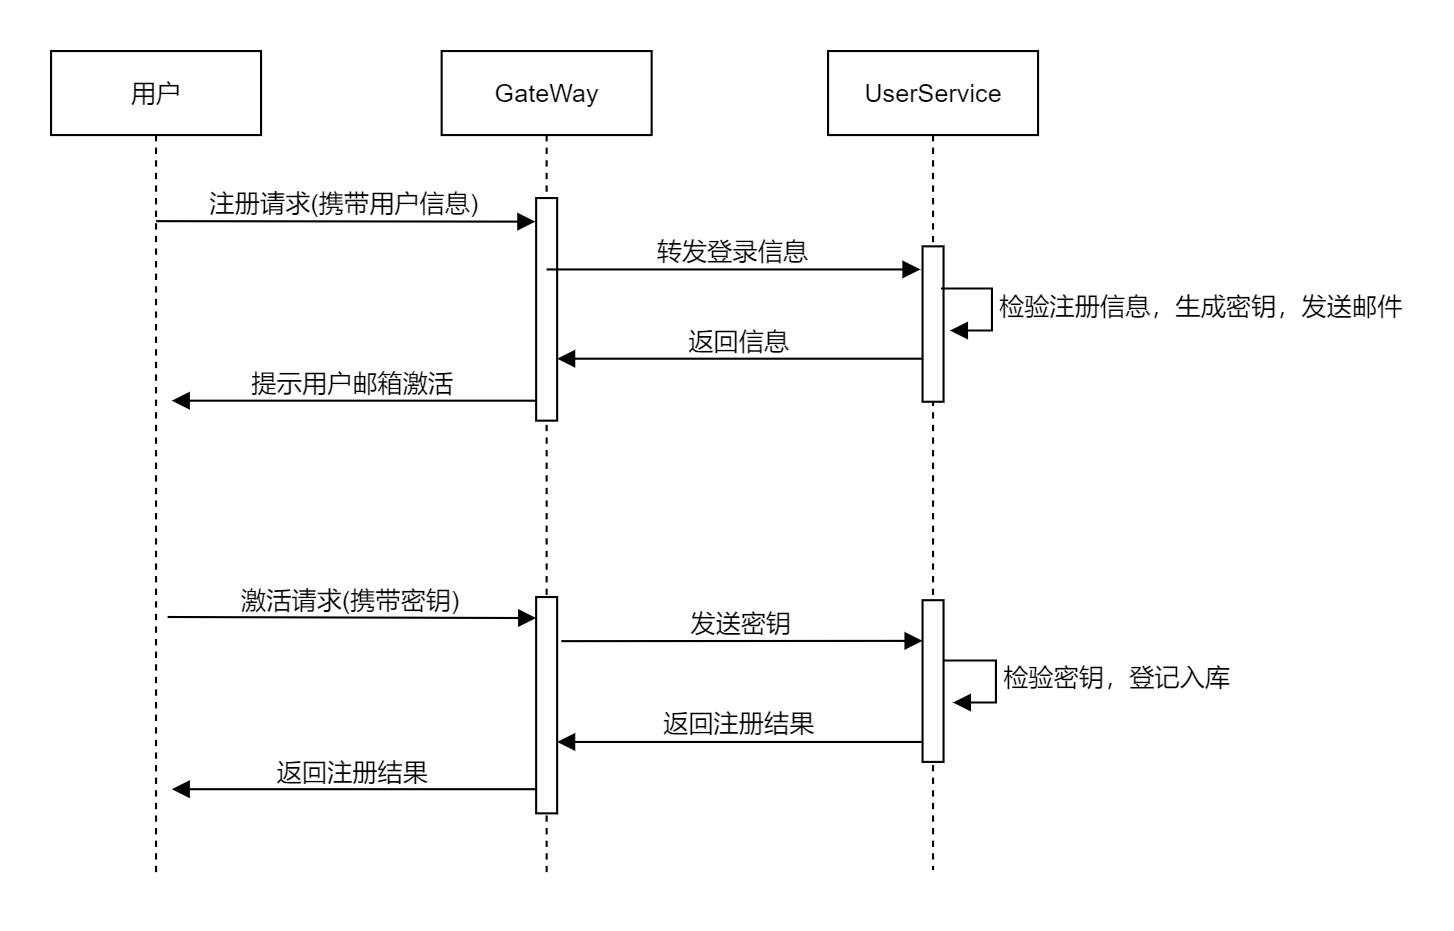
\includegraphics[width=\textwidth]{ch7/register.jpg}
    \caption{注册授权}\label{fig:register}
    \vspace{\baselineskip} % 表示图与正文空一行
\end{figure}

\subsection{用户发布房源贴}
用户在房源系统中发布房源援助帖子,同时需要选择标签和联系方式。只有经过实名安全认证过的用户才能进行房源发布,实名安全认证服务有第三方提供。

具体流程为:
\begin{itemize}
    \item 用户请求发帖接口,网关转发注册信息至房源管理模块。
    \item 房源接口检验参数合法性,不合法则返回发帖失败信息。
    \item 合法则将信息入库,并将发帖成功信息返回给客户端。
\end{itemize}

下图图~\ref{fig:launchpost}~为时序图:
\begin{figure}[htbp]
    \centering
    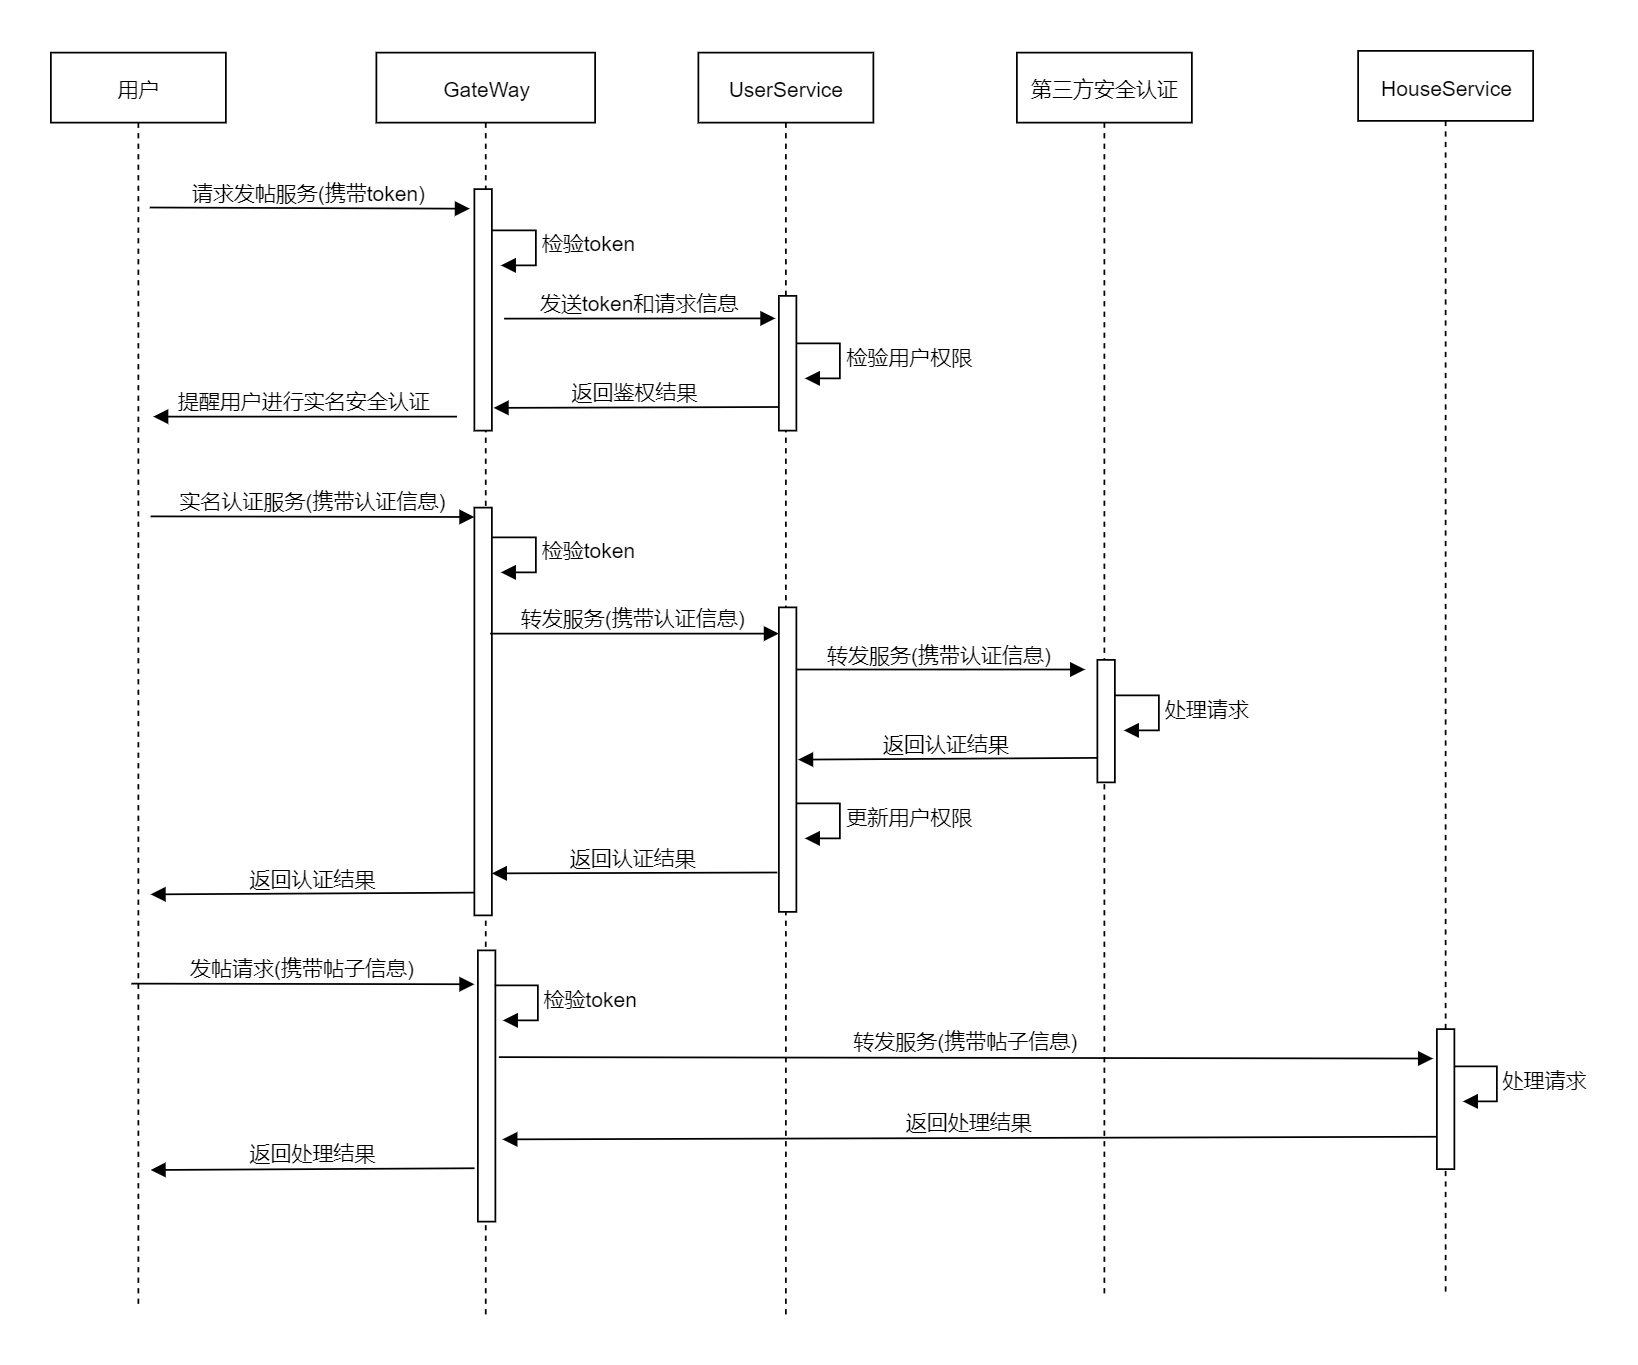
\includegraphics[width=\textwidth]{ch7/launchpost.jpg}
    \caption{用户发布房源帖}\label{fig:launchpost}
    \vspace{\baselineskip} % 表示图与正文空一行
\end{figure}

\subsection{管理员进行用户管理}
管理进行用户管理时,首先需要用户服务模块检验管理员的权限,权限通过后管理员可以对用户进行操作。比如冻结或解冻用户,剥夺用户权限等等。同时,管理员的
每次操作都需要载入日志。同时,系统会给帖子用户发送通知。

具体流程为:
\begin{itemize}
    \item 管理员请求用户管理接口,网关转发请求信息至用户管理模块。
    \item 用户模块检验管理员身份和权限,通过则继续执行操作,否则返回权限不足。
    \item 用户模块执行用户管理操作,并生成日志信息,封装转发给系统服务模块。
    \item 系统服务接收服务信息,校验参数,写入日志数据库,同时发送通知给相关用户。
\end{itemize}

下图图~\ref{fig:admin-user}~为时序图:
\begin{figure}[htbp]
    \centering
    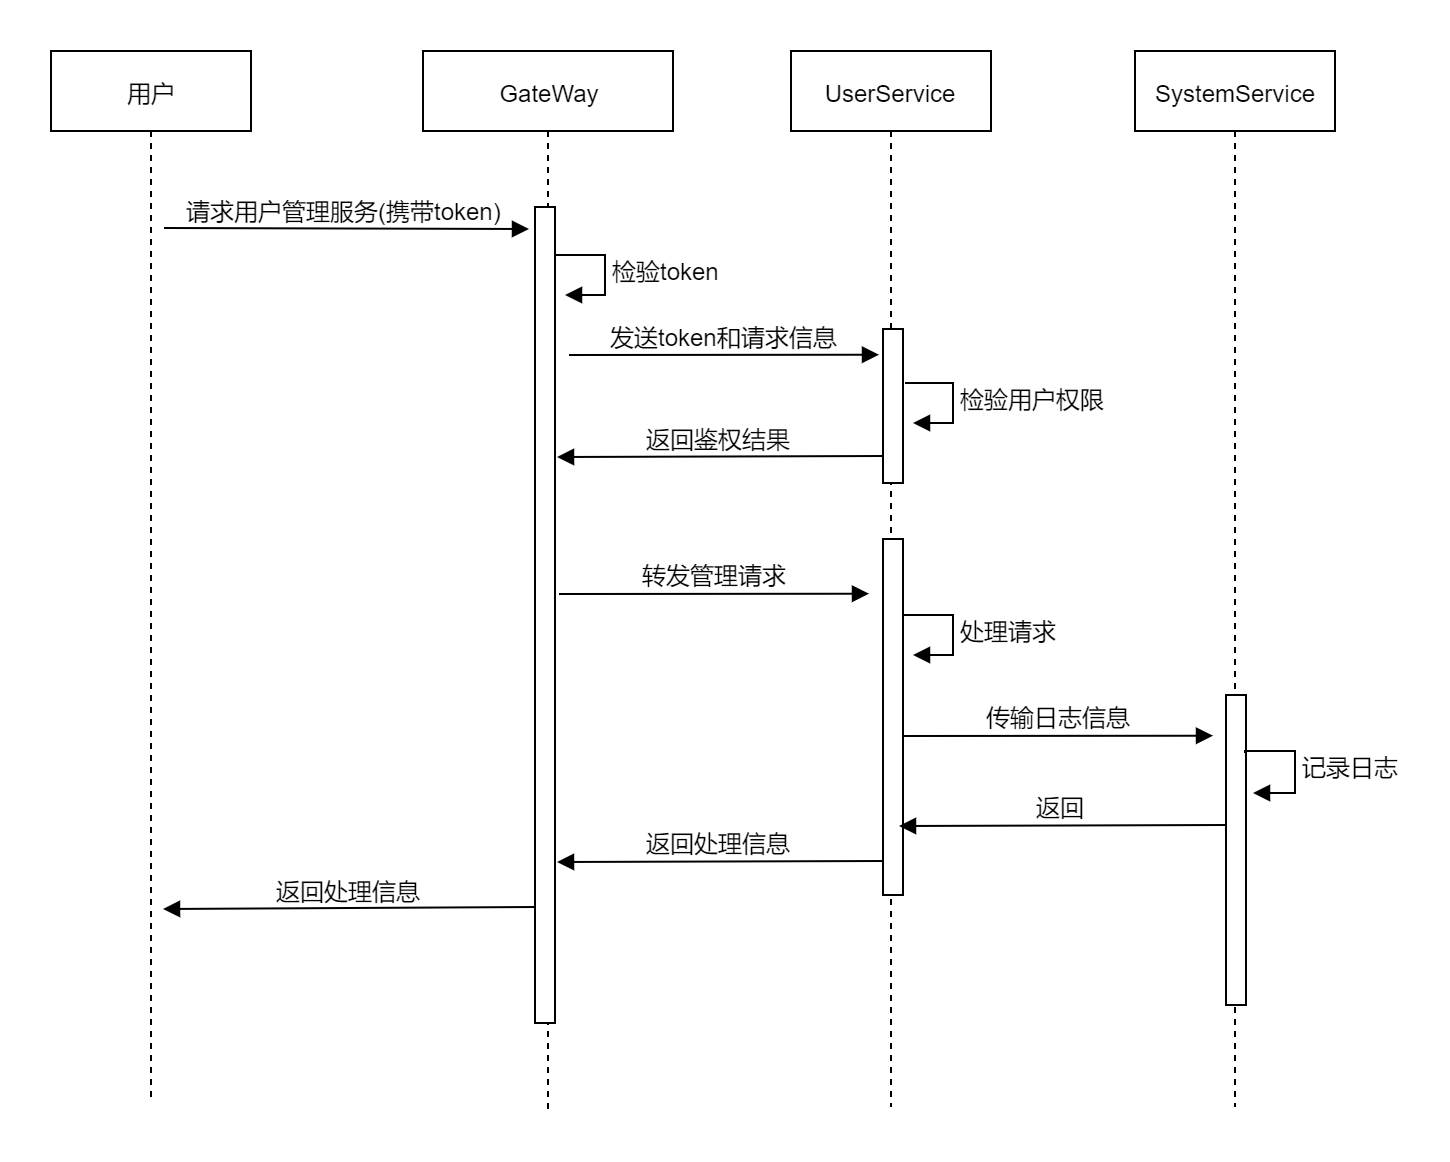
\includegraphics[width=\textwidth]{ch7/admin-user.jpg}
    \caption{管理员用户管理}\label{fig:admin-user}
    \vspace{\baselineskip} % 表示图与正文空一行
\end{figure}

\subsection{管理员进行房源管理}
管理进行房源管理时,首先需要用户服务模块检验管理员的权限,权限通过后管理员可以对帖子进行操作。比如删除帖子等。同时,管理员的
每次对帖子操作会生成日志文件,交由系统处理。同时,系统会给帖子用户发送通知。

具体流程为:
\begin{itemize}
    \item 管理员请求帖子管理接口,网关转发请求信息至用户管理模块。
    \item 用户模块检验管理员身份和权限,通过则转发请求给房源系统,否则返回权限不足。
    \item 房源模块执行帖子管理操作,并生成日志信息,封装转发给系统服务模块。
    \item 系统服务接收服务信息,校验参数,写入日志数据库,同时发送通知给相关用户。
\end{itemize}

下图图~\ref{fig:admin-post}~为时序图:
\begin{figure}[htbp]
    \centering
    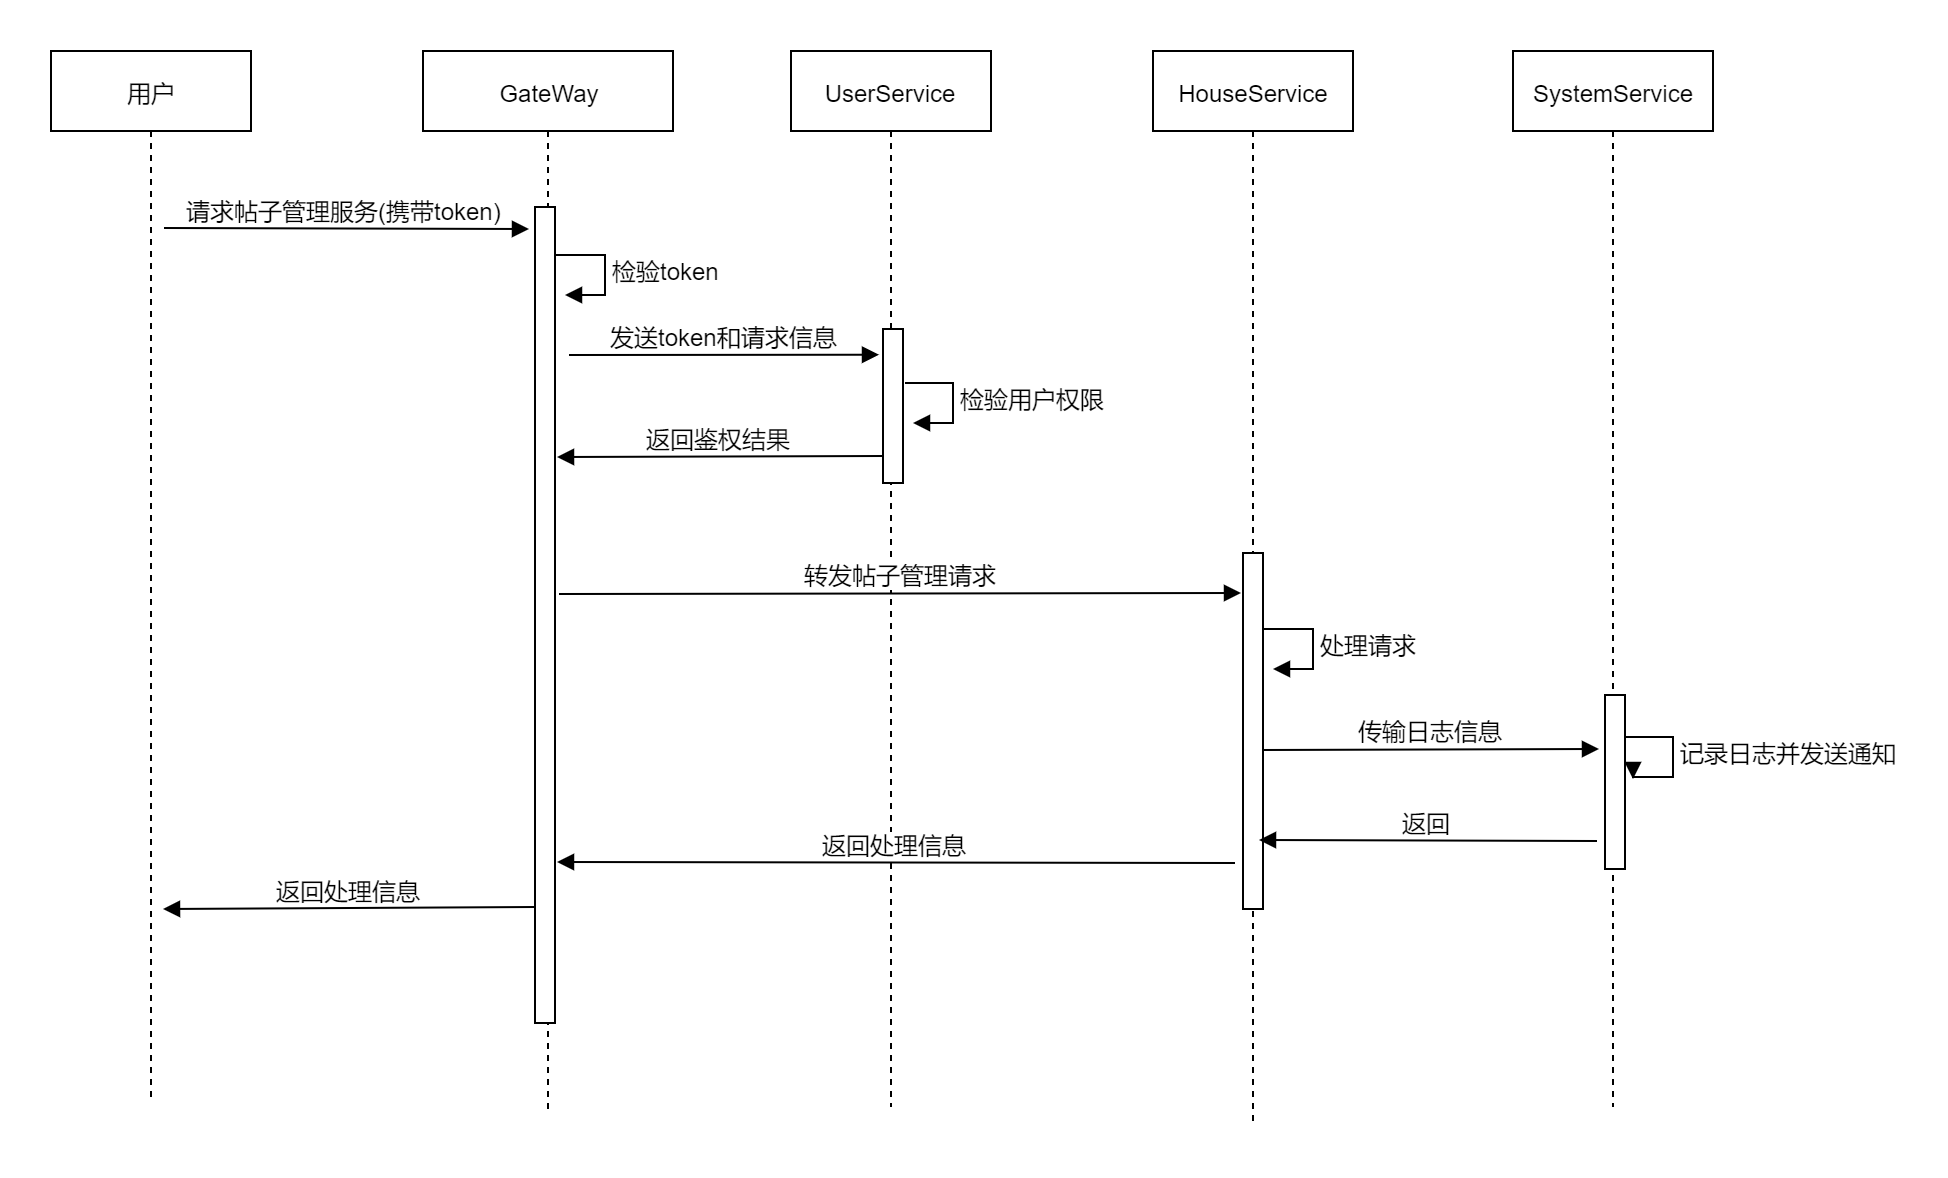
\includegraphics[width=\textwidth]{ch7/admin-post.jpg}
    \caption{管理员帖子管理}\label{fig:admin-post}
    \vspace{\baselineskip} % 表示图与正文空一行
\end{figure}

\subsection{管理员进行新闻管理}
管理进行新闻管理时,首先需要用户服务模块检验管理员的权限,权限通过后管理员可以对新闻进行操作。比如删除新闻等。同时,管理员的
每次对新闻操作会生成日志文件,交由系统处理。同时,系统会给相关编辑者发送通知。

具体流程为:
\begin{itemize}
    \item 管理员申请新闻管理接口,网关转发请求信息至用户管理模块。
    \item 用户模块检验管理员身份和权限,通过则继续转发给新闻模块,否则返回权限不足。
    \item 新闻模块执行新闻管理操作,并生成日志信息,封装转发给系统服务模块。
    \item 系统服务接收服务信息,校验参数,写入日志数据库,同时发送通知给相关用户。
\end{itemize}

下图图~\ref{fig:admin-news}~为时序图:
\begin{figure}[htbp]
    \centering
    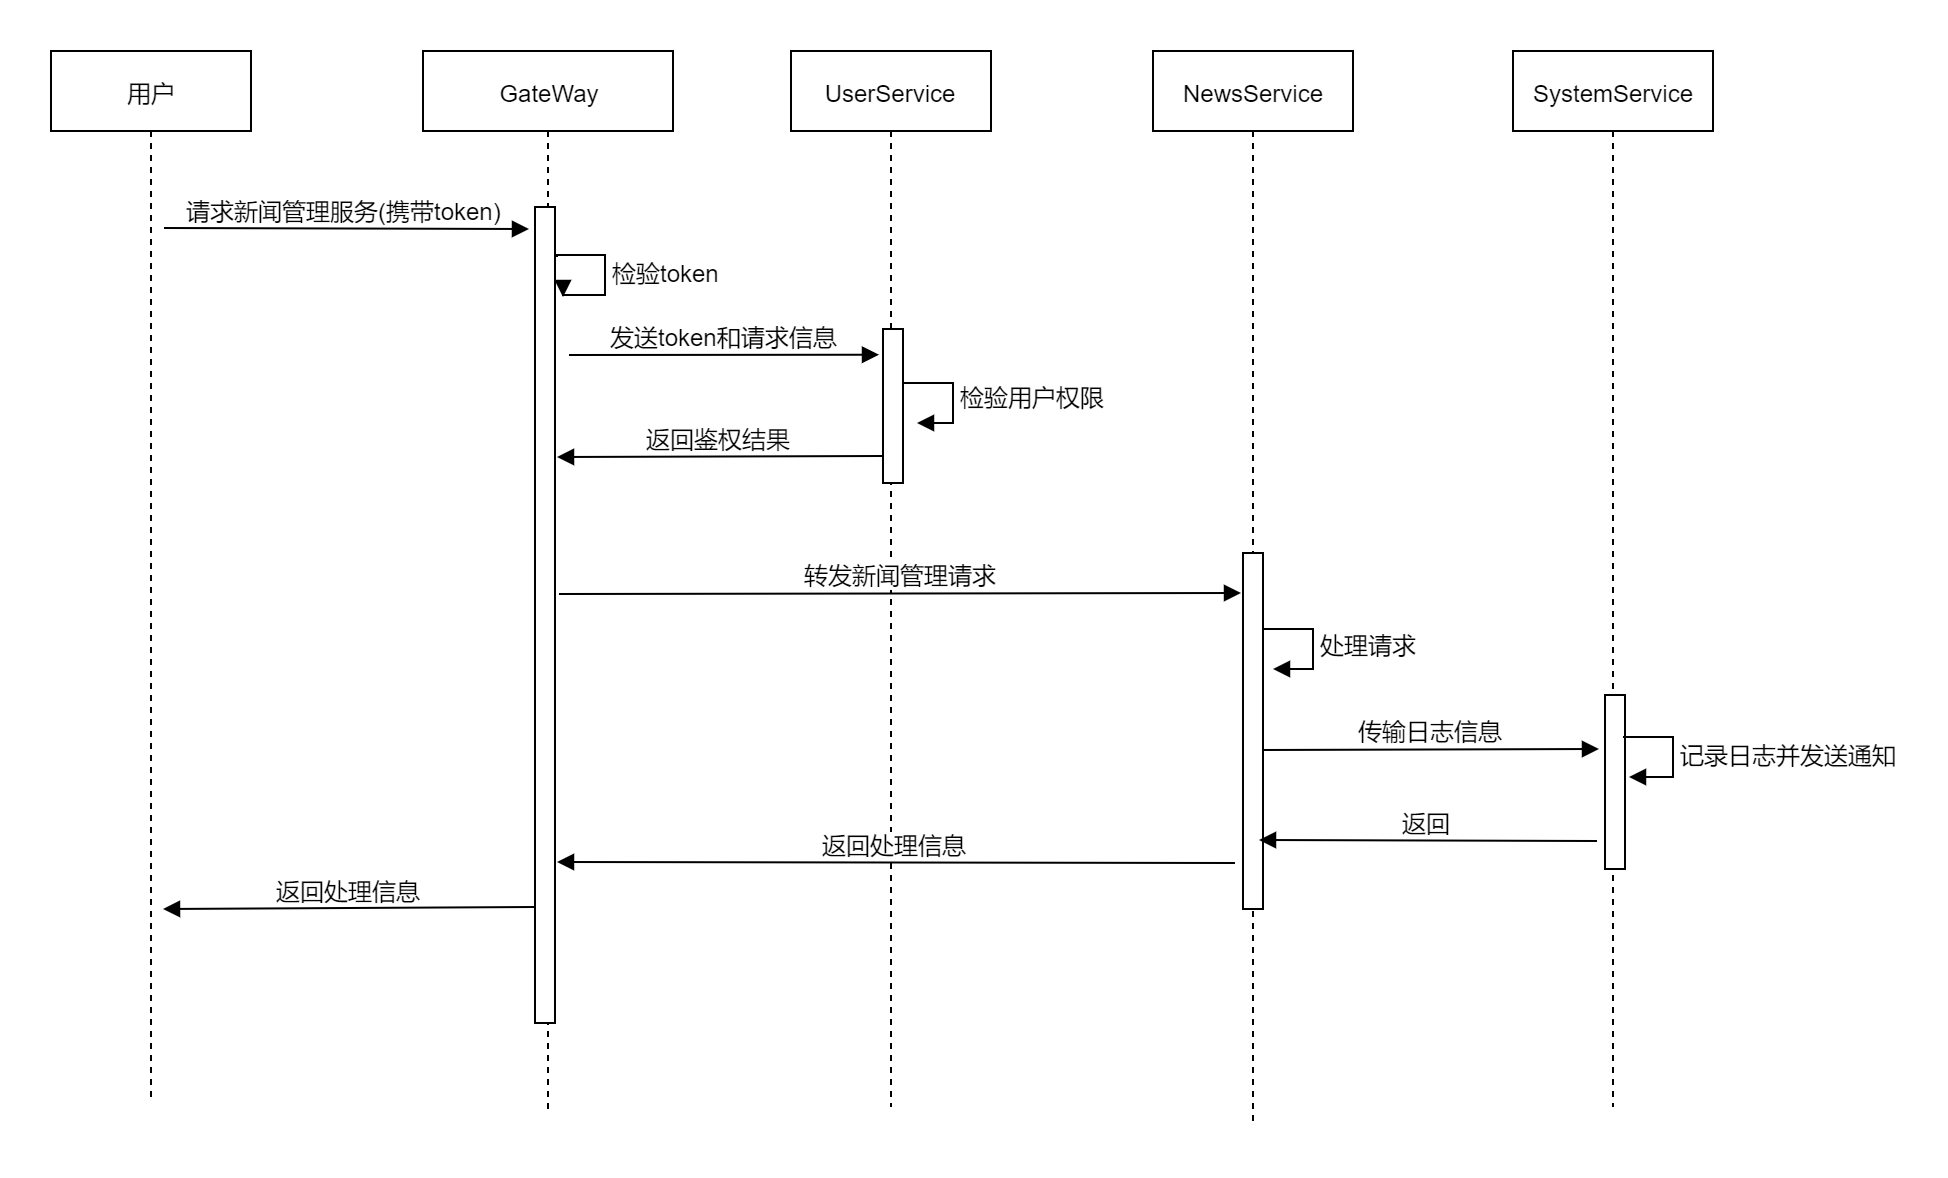
\includegraphics[width=\textwidth]{ch7/admin-news.jpg}
    \caption{管理员新闻管理}\label{fig:admin-news}
    \vspace{\baselineskip} % 表示图与正文空一行
\end{figure}

\subsection{管理员审核举报}
管理员进行举报审核时,首先需要用户服务模块检验管理员的权限,权限通过后管理员可以对举报进行审核,比如通过和驳回等。同时,管理员的
每次对审核操作会生成日志文件,交由系统处理。同时,系统会给相关编辑者发送通知。

具体流程为:
\begin{itemize}
    \item 管理员申请举报审核接口,网关转发请求信息至用户管理模块。
    \item 用户模块检验管理员身份和权限,通过则继续转发给审核模块,否则返回权限不足。
    \item 审核模块处理后生成举报修改类,向举报模块发送修改举报状态的请求。
    \item 审核模块生成日志信息,封装转发给系统服务模块。
    \item 系统服务接收服务信息,校验参数,写入日志数据库,同时发送通知给相关用户。
\end{itemize}

下图图~\ref{fig:audit-report}~为时序图:
\begin{figure}[htbp]
    \centering
    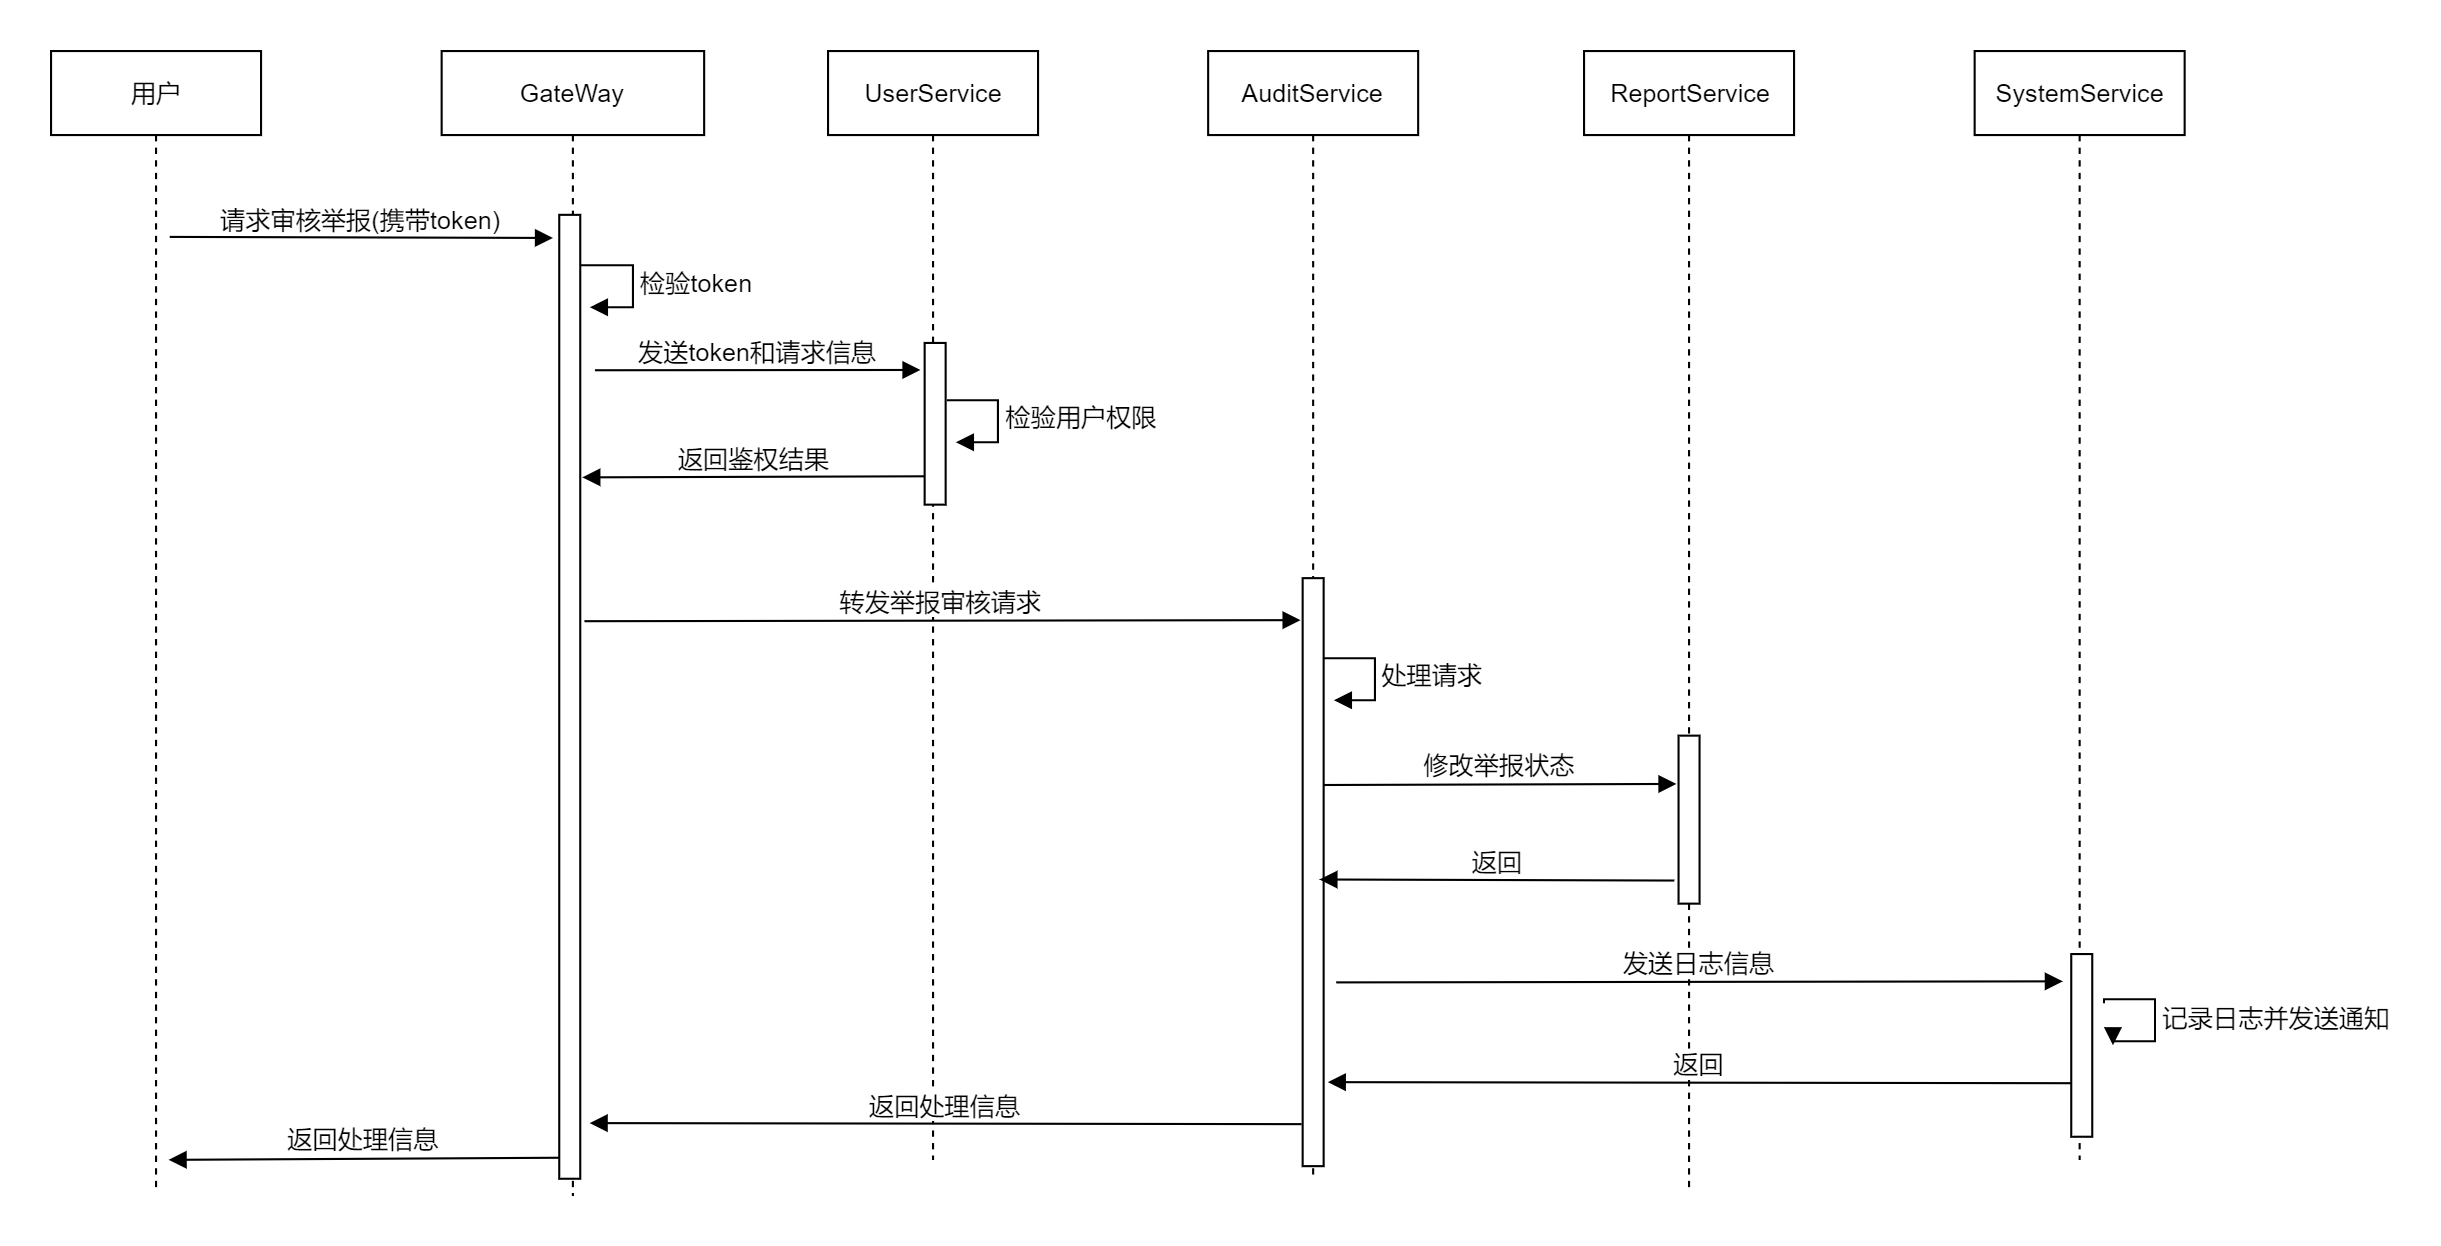
\includegraphics[width=\textwidth]{ch7/audit-report.jpg}
    \caption{管理员审核举报}\label{fig:audit-report}
    \vspace{\baselineskip} % 表示图与正文空一行
\end{figure}

\subsection{管理员审核新闻}
管理员进行审核新闻时,首先需要用户服务模块检验管理员的权限,权限通过后管理员可以对新闻进行审核,比如通过和驳回等。同时,管理员的
每次对审核操作会生成日志文件,交由系统处理。同时,系统会给相关编辑者发送通知。

具体流程为:
\begin{itemize}
    \item 管理员申请新闻审核接口,网关转发请求信息至用户管理模块。
    \item 用户模块检验管理员身份和权限,通过则继续转发给审核模块,否则返回权限不足。
    \item 审核模块处理后生成新闻修改类,向新闻模块发送修改新闻状态的请求。
    \item 审核模块生成日志信息,封装转发给系统服务模块。
    \item 系统服务接收服务信息,校验参数,写入日志数据库,同时发送通知给相关用户。
\end{itemize}

下图图~\ref{fig:audit-news}~为时序图:
\begin{figure}[htbp]
    \centering
    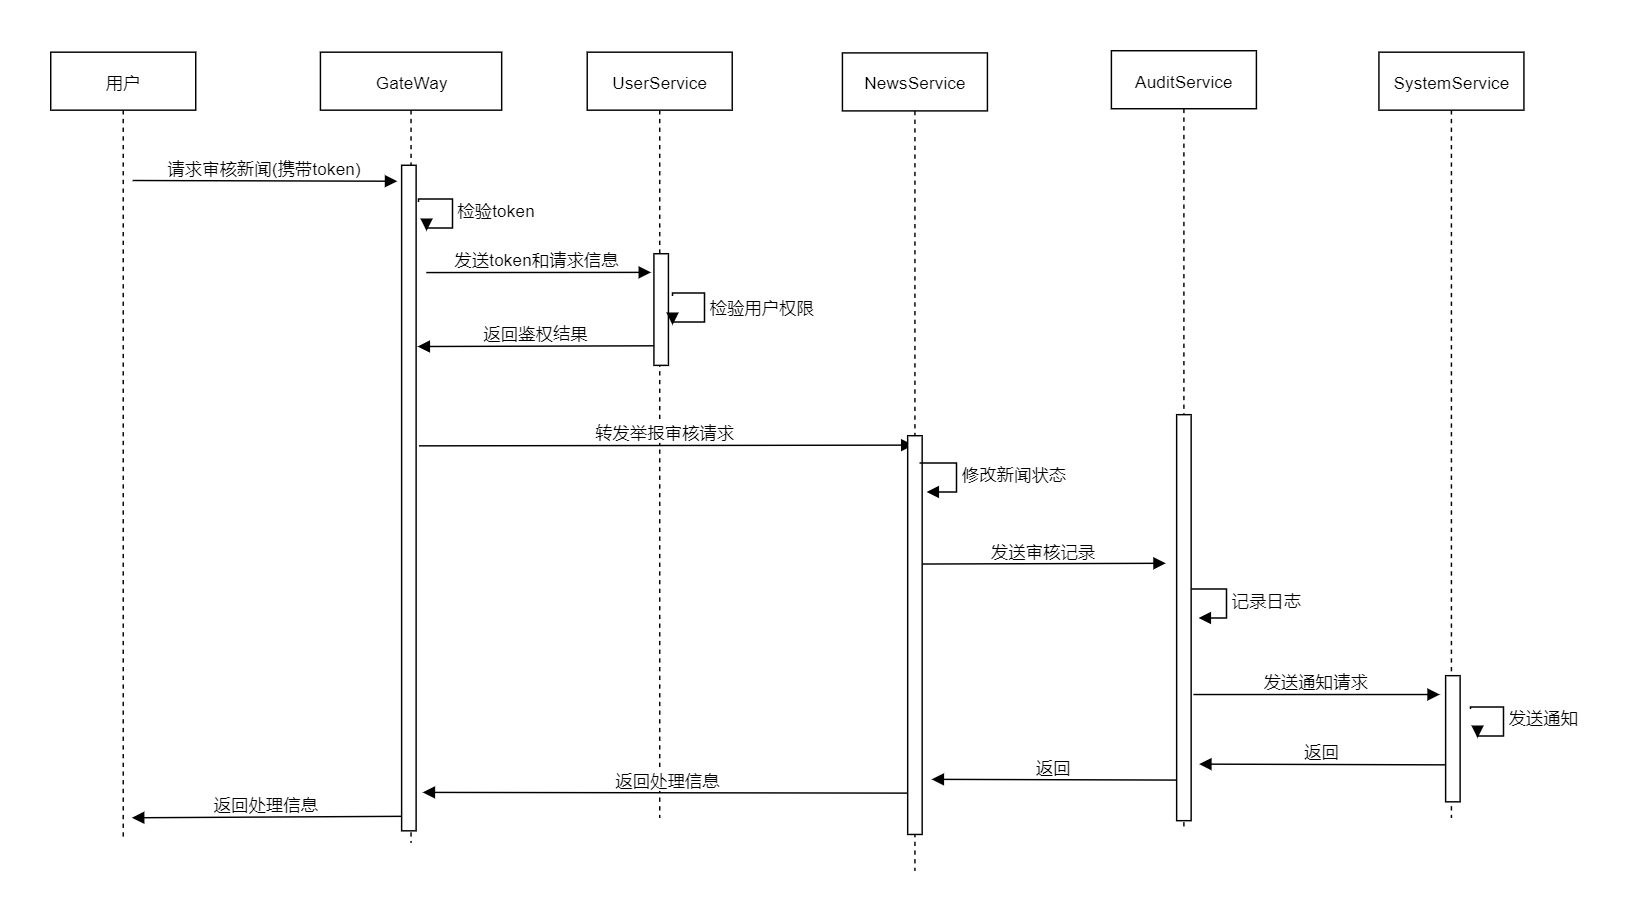
\includegraphics[width=\textwidth]{ch7/audit-news.jpg}
    \caption{管理员审核新闻}\label{fig:audit-news}
    \vspace{\baselineskip} % 表示图与正文空一行
\end{figure}







